\section{Overview}
\label{sec:overview}%
Here we represent an overview of how the entire S\&C architecture is composed of:

\begin{figure}[H]
    \begin{center}
        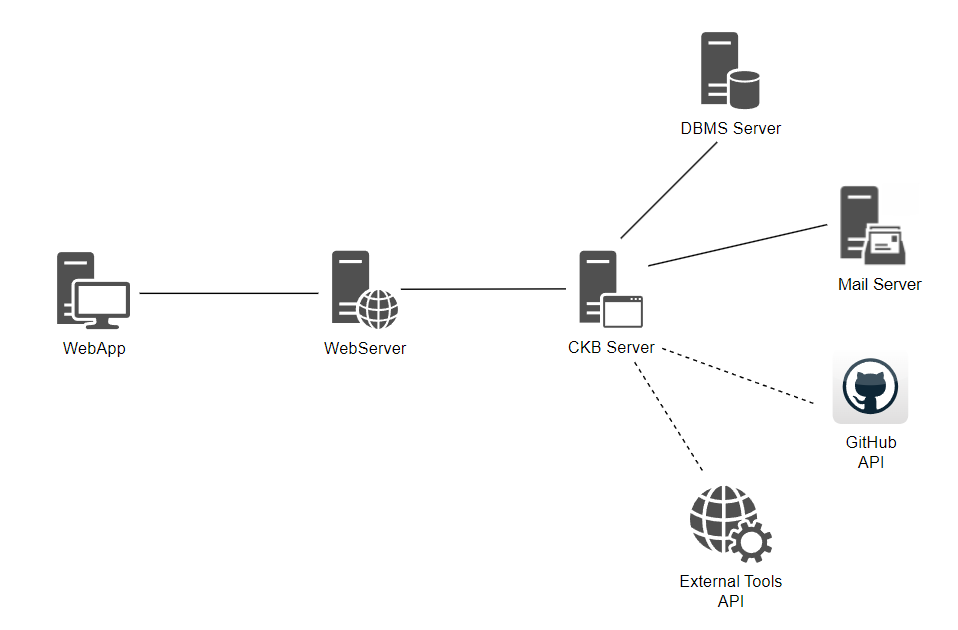
\includegraphics[width=1\linewidth]{CD_DD/Overview.png}
        \caption{S\&C Overview.}
        \label{fig:CKB_overview}%
    \end{center}
\end{figure}

\noindent Client side:
\begin{itemize}
    \item WebApp: Represents the User Interface of the system, providing access through a web application to the offered services such as registration, login, updating profile overview, creating internships, searching and applying for internships, creating tasks for candidates, submitting complaints or providing feedback. It’s responsible for all the User interactions, and it communicates with the main server through the Web Server, using secure protocols like HTTPS.
\end{itemize}
\noindent Server side:
\begin{itemize}
    \item \textbf{Web Server:} handles communication with Users, receiving and processing their inputs. Additionally, it provides load balancing for requests, distributing them among various replicas of the S\&C Server. It also manages the User sessions.
    \item \textbf{S\&C Server:} the core of the system, contains most of the logic of the software and handles interactions between different components. It also coordinates the communication with the DBMS, triggers the recommendation algorithm through the External Tools API and sends notifications to the users. It serves as the primary server for the entire website and is replicated across multiple machines to handle a high volume of requests.
    \item \textbf{DBMS Server:} stores data related to Users, Internships, Resumes, Complaints and Feedback. It acts as the repository for essential information.
    \item \textbf{Mail Server:} is responsible for sending confirmation email when a new User registers on S\&C, enhancing the User registration process.
    \item \textbf{External Tools API:} used to run the recommendation algorithm. It also takes feedback in inputs to reinforce the algorithm over time, ensuring better accuracy in the matching process.
\end{itemize}

\section{Component View}
\label{sec:component_view}%

\subsection{High Level Diagram}
\label{subsec:high_level_diagram}%

\begin{figure}[H]
    \begin{center}
        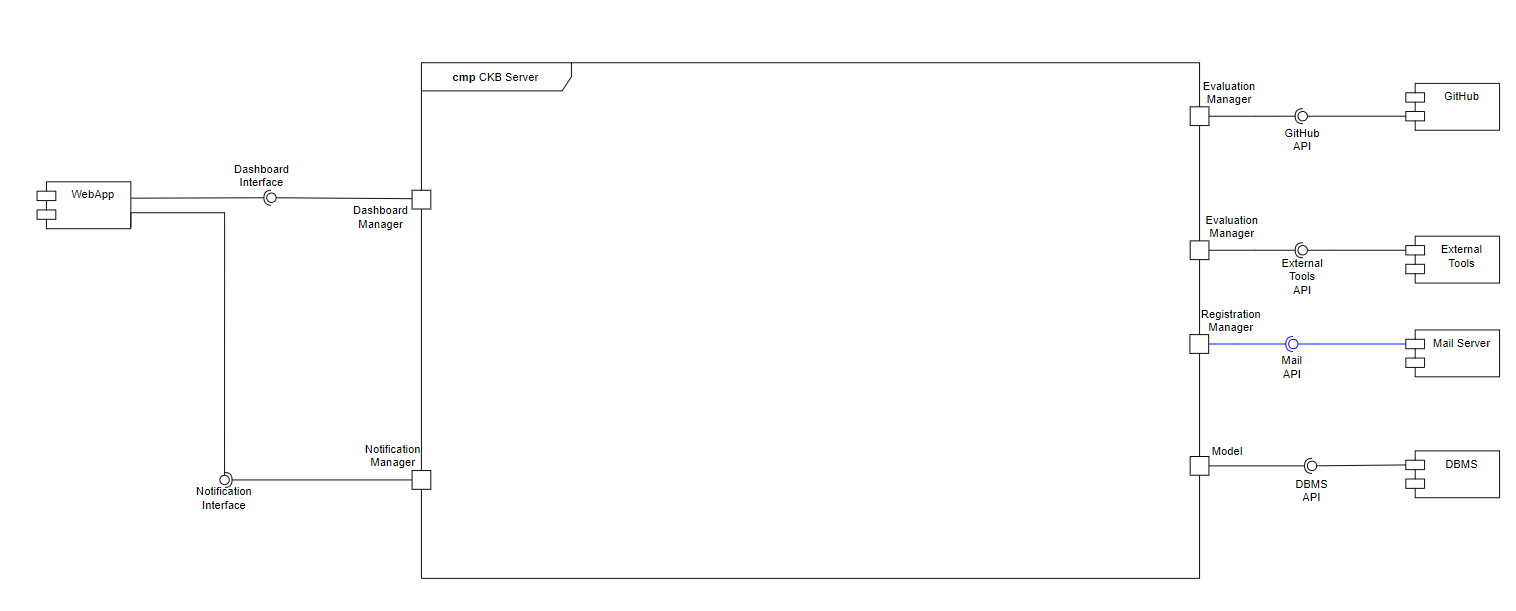
\includegraphics[width=1\linewidth]{CD_DD/HighLevel.png}
        \caption{High Level Diagram.}
        \label{fig:high_level_diagram}%
    \end{center}
\end{figure}

\noindent In the figure above is the high level component diagram of S\&C where it’s represented the external components of S\&C and how they communicate with the S\&C server, in particular:
\begin{itemize}
    \item \textbf{WebApp}: serves as the external access point for Users, allowing communication with the S\&C Server through the Dashboard Interface—the sole means for Client-Server interaction from the User side. The S\&C Server can relay notifications, such as Student uploading overviews or Internship creation, to Users through the Notification Interface.
    \item \textbf{DBMS:} is the storage repository for all User data, Internships, Feedback and Complaints. It communicates with the S\&C Server via the DBMS API, which is connected to the Model component.
    \item \textbf{Mail Server:} responsible for sending registration confirmation emails, the Mail Server communicates with the S\&C Server using the Mail API interface. This interface is linked to the Registration Manager component, which oversees the User registration process..
    \item \textbf{External Tools:} external application used for running and reinforcing a sophisticated recommendation algorithm. It communicates with the S\&C Server through the External Tools API, connecting to the Recommendation Manager component. The Recommendation Manager handles the notification process for the matching phase of the system.
\end{itemize}

\subsection{Low Level Diagram}
\label{subsec:low_level_diagram}%

\begin{figure}[H]
    \begin{center}
        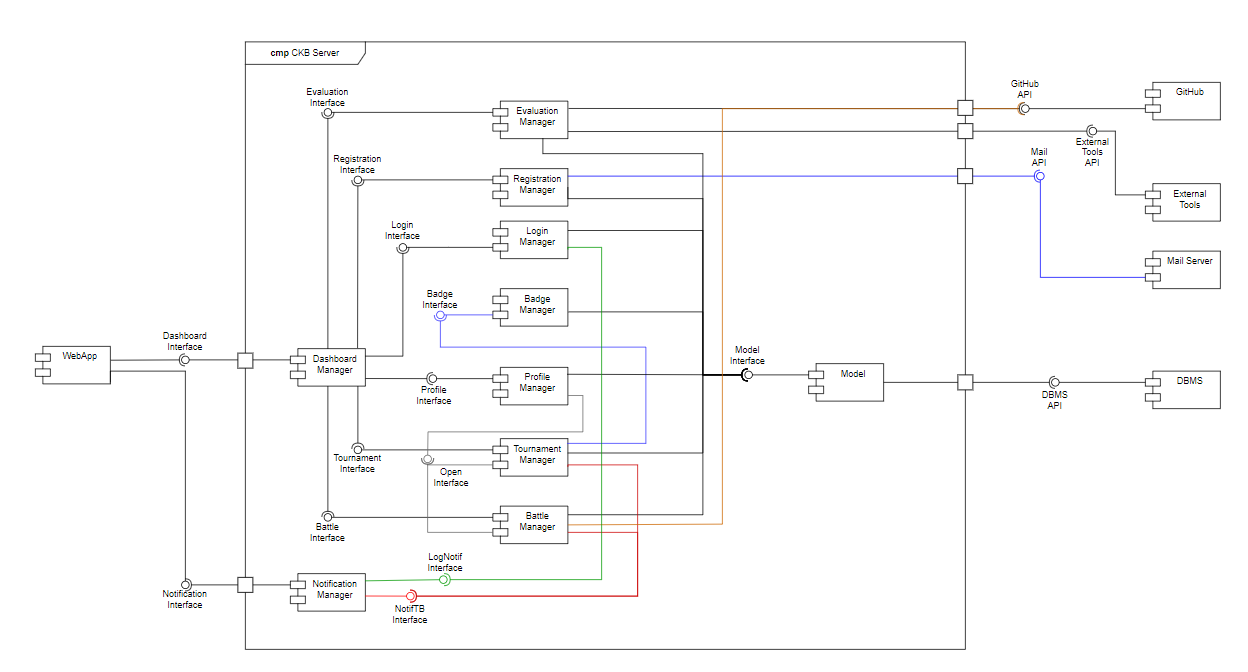
\includegraphics[width=1\linewidth]{CD_DD/LowLevel.png}
        \caption{Low Level Diagram.}
        \label{fig:low_level_diagram}%
    \end{center}
\end{figure}

\noindent The figure above represents the complete architecture of S\&C website with each components inside the S\&C Server:
\begin{itemize}
    \item \textbf{Dashboard Manager:} This fundamental component orchestrates all the communication between User and the S\&C website. Users communicate with the system through the Dashboard Interface, so the Dashboard Manager address all the requests to the right component, depending on the User's needs. 
    \item \textbf{Model:} This component represents the dataset of the server, and it act as a mask to the database server, so every component have to interface with it to access data from DBMS, which will access it directly through the DBMS API. 
    \item \textbf{Recommendation Manager:}  The component that handles everything about the recommendation phase of the system. It periodically triggers a new computation for finding new matches between students and internships, and it does that by using the External Tools API, which communicates directly with the system in which the computation take place. It also communicate with the model for retrieving all the information necessary to the user to visualize the correct recommendation list, each time there is a new request incoming from the Dashboard Manager. This component additionally communicates with the Profile Manager through the View Profile Interface, every time that a company, from it's recommendation list wants to check the profile overview of a Student.
    \item \textbf{Registration Manager:} This components handles the registration of new Users on the system. The User when trying to create a new account interacts with the Dashboard Manager, which contacts the Registration Manager through the Registration interface. Then the Registration Manager handle the request and manages to contact the Mail Server through the Mail API, to send a confirmation email to the new User. Once this is done it uses the Model through the Model Interface for saving user's information on the DBMS.
    \item \textbf{Login Manager:} This component handle the Login process for registered Users. When a User attempts to Login, the Dashboard Manager address the request to this component, which contacts the Model through the Model Interface to retrieve data from the DBMS and so authenticate the User. 
    \item \textbf{Profile Manager:} Component that allows Students to create their profile overview. When a Student starts the process to complete it's profile, the Dashboard Manager forwards the requests to the Profile manager using the Profile Interface. The Profile Manager communicates with the Model component through the Model Interface to store new information in the DBMS. It also manage to retrieve Students information when a company wants to view the overview of a Student within the recommendation list.
    \item \textbf{Internship Manager:} This component allow the Companies to create, modify and visualize internships. When a company wants to publish a new internship, interacts with the dashboard manager, which forwards the requests to the Internship Manager. This component manage to save new published internship, modify the status or retrieve information for internship search from the Model component, interacting with it via the Model Interface.
    \item \textbf{Interview Manager:} This is the main component of the interview phase of an internship. When a company wants to start preparing tasks or submit them to candidates, interacts with the Dashboard Manager, who forwards the requests to the Interview Manager, who manage to interact with the Model through the Model Interface for saving information. It can also notify the candidates when the tasks are ready to be carried out, or results are ready, contacting the Notification Manager module through the InterviewNotif Interface.
    \item \textbf{Complaints Manager:} This component handles the complaints related to an internship. When a User wants to file a complaint about an internship, interact with the Dashboard Manager, who forwards the requests to the Complaint Manager through the Complaint Interface, which needs to Notify the University of the Student related complaint, contacting the Notification Manager module through the InterviewNotif Interface. It can also store the complaints on the model for the purpose of reinforcing the algorithm.
    \item \textbf{Notification Manager:} Component that handles each notification that has to be sent to the Users, in particular when a new match has been found from the recommendation algorithm, it sends a notification both to the Student and the Company related with that match; when the interview phase is completed, it sends the notification to all the candidates informing them wether they've been selected or not; when a new complaint is made from a company or a student, it notify the university that has to handle it. All the communication from other components to this are made through the InterviewNotif Interface, ComplNotif Interface or the Recommendation Interface, and it communicates with the web app through the Notification Interface..
\end{itemize}

\subsection{Recommendation Manager}
\label{subsec:recommendation_manager}%

\begin{figure}[H]
    \begin{center}
        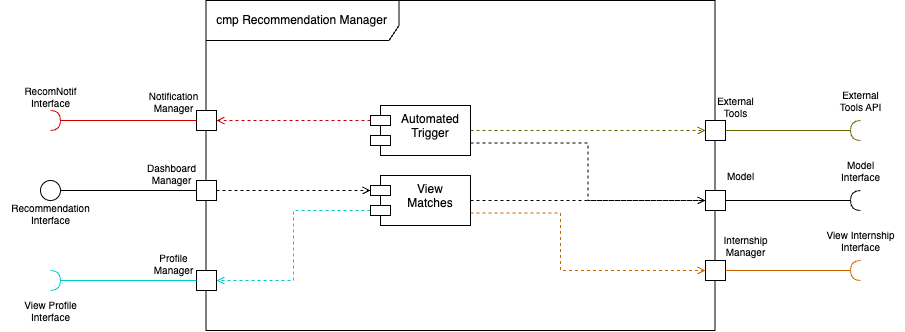
\includegraphics[width=1\linewidth]{CD_DD/RecommendationManager.png}
        \caption{Recommendation Manager.}
        \label{fig:recommendation_manager}%
    \end{center}
\end{figure}

\noindent The Recommendation Manager is composed by two other sub-components, one for handling the automated trigger for the recommendation algorithm and the other one for showing to the user their recommendation list:

\begin{itemize}
    \item \textbf{Automated Trigger component:} This component is essential for ensuring the continuous and autonomous operation of the recommendation system. Its primary function is to periodically initiate the recommendation algorithm, which scans the database for new or updated profiles and internship postings. By doing so, the component guarantees that students and companies receive the most relevant and recent matches based on evolving criteria such as updated CVs, new internship opportunities, and feedback collected from previous experiences. This component interfaces directly with the External Tools API, responsible for executing the complex matching logic that considers various parameters, including skills, interests, and project domains.
    \item \textbf{View Matches component:} The View Matches component retrieves the latest matches identified by the Automated Trigger and displays them through the user’s dashboard. For students, a list of internship opportunities that align with their skills and interests. For companies, potential candidates whose profiles closely match the requirements of their internship postings. Users can also filter and sort recommendations. Additionally, the View Matches component provides direct links to student profiles or internship details.
\end{itemize}

\subsection{Internship Manager}
\label{subsec:internship_manager}%

\begin{figure}[H]
    \begin{center}
        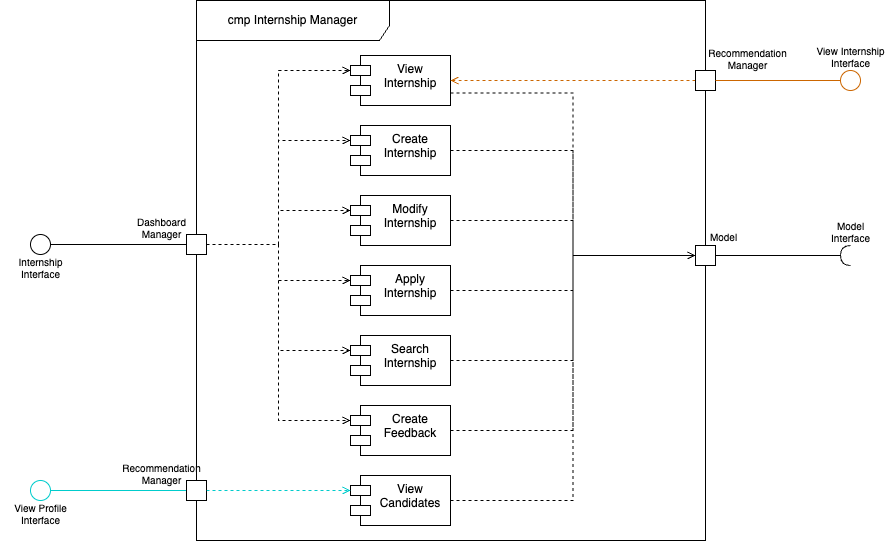
\includegraphics[width=1\linewidth]{CD_DD/InternshipManager.png}
        \caption{Internship Manager.}
        \label{fig:internship_manager}%
    \end{center}
\end{figure}

\noindent The Internship Manager is made by the following components:

\begin{itemize}
    \item \textbf{View internship component:} The View Internship component provides a comprehensive interface for accessing and managing internship postings within the system. For students, the component acts as a searchable catalogue of available internships, with filtering and sorting options. This component pulls data directly from the DBMS through the Model Interface, ensuring real-time synchronization with the latest postings. It allows companies to view the number of applicants, monitor engagement, and update internship details if necessary. For students, each internship listing includes detailed descriptions, project requirements, and any associated benefits. Additionally, the View Internship component integrates with the Apply Internship subcomponent.
    \item \textbf{Create internship component:} This component facilitates the creation and publication of new internship offers by companies. It provides a structured form that guides users through defining essential parameters, such as internship title, required skills, project description, duration, and compensation details. Once the form is completed, the Create Internship component validates the input to ensure completeness and consistency. It then interfaces with the DBMS through the Model component to store the new internship in the database. If errors are detected during the validation process, the component provides immediate feedback, allowing the user to correct any issues before submission.
    \item \textbf{Modify internship component:} The Modify Internship component enables companies to update or delete existing internship postings. Users can access this component through the View Internship interface, selecting the internship they wish to edit. Changes made through the Modify Internship component are instantly propagated to the DBMS, ensuring all users view the most up-to-date information. 
    \item \textbf{Apply internship component:} The Apply Internship component is central to the student experience on the platform. It allows students to submit applications for internships directly through the system. Upon clicking the “Apply” button, the component gathers the student’s profile data, CV, and any additional required documents before forwarding the application to the target company. Companies are notified of new applications via the Notification Manager, ensuring timely review and response. The Apply Internship component also includes mechanisms for students to withdraw applications if necessary, with relevant notifications sent to the company and the system updated accordingly.

    \item \textbf{Create feedback component:} After an internship is completed, the Create Feedback component enables students and companies to provide feedbacks about their experience. Companies evaluate student performance, highlighting strengths and areas for improvement. Similarly, students can rate their experience with the company, providing insights into the quality of mentorship, project alignment, and overall satisfaction. This component compiles feedback into structured reports, which are stored in the DBMS. The feedback serves as valuable input for refining the recommendation algorithm, improving the accuracy of future matches by incorporating performance data and user satisfaction.
    \item \textbf{View Candidates component:} This component allows companies to access and manage the list of students who have applied for their internships. Through an interactive dashboard, companies can view applicant profiles, download CVs, and review additional submitted documents. The component includes sorting and filtering tools. Additionally, it provides features for marking applicants as shortlisted, rejected, or accepted. Once candidates are selected, the component forwards their details to the Interview Manager, initiating the next phase of the recruitment process. Notifications are sent to the selected students, informing them of their application status.
\end{itemize}

\subsection{Profile Manager}
\label{subsec:profile_manager}%

\begin{figure}[H]
    \begin{center}
        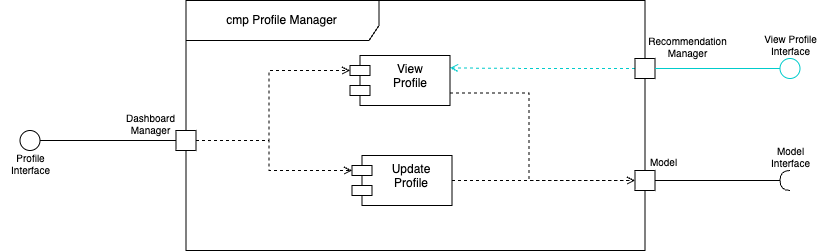
\includegraphics[width=1\linewidth]{CD_DD/ProfileManager.png}
        \caption{Profile Manager.}
        \label{fig:profile_manager}%
    \end{center}
\end{figure}

\noindent The Profile Manager is the component :

\begin{itemize}
    \item \textbf{View Profile component:} The View Profile component allows users to access and review profiles stored within the system. For students, this component displays their profile overview, including personal information, educational background, skills, and uploaded CVs. For companies, it provides access to student profiles that match internship postings or appear on recommendation lists. The component supports viewing profiles in detail and exporting them for offline review. The View Profile component integrates directly with the DBMS to ensure that profile data is current and reflective of the latest updates made by students.
    \item \textbf{Update Profile component:} This component is designed to enable students to manage and update their profiles. Students can edit sections related to personal details, work experience, skills, and education. The Update Profile component performs real-time validation to ensure that all data entered adheres to format and completeness standards. Once submitted, the updated data is written to the DBMS via the Model component. The system also supports partial updates, allowing students to save progress and complete their profiles incrementally.
\end{itemize}

\subsection{Complaints Manager}
\label{subsec:complaints_manager}%

\begin{figure}[H]
    \begin{center}
        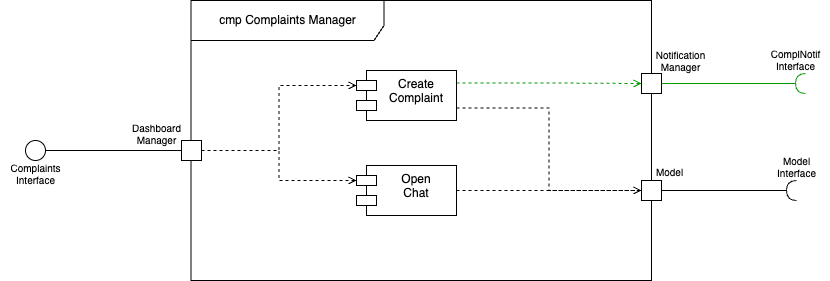
\includegraphics[width=1\linewidth]{CD_DD/ComplaintsManager.png}
        \caption{Complaints Manager.}
        \label{fig:complaints_manager}%
    \end{center}
\end{figure}

\noindent The Complaints Manager is the component :

\begin{itemize}
    \item \textbf{Create Complaint component:} The Create Complaint component allows users to file formal complaints about internships. This feature is available to both students and companies, providing a structured form to capture detailed descriptions of issues encountered during the internship process. The component sends complaints to the relevant university, which is notified through the Notification Manager. Complaints are logged in the DBMS, ensuring traceability and enabling further investigation if needed.
    \item \textbf{Open Chat component:} This component facilitates direct communication between universities and users regarding complaints. It opens a secure chat channel, allowing real-time interaction to resolve issues efficiently.
\end{itemize}

\subsection{Application Manager}
\label{subsec:application_manager}%

\begin{figure}[H]
    \begin{center}
        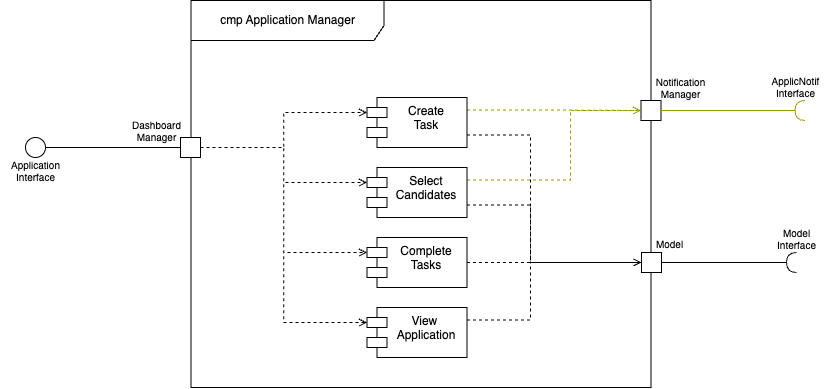
\includegraphics[width=1\linewidth]{CD_DD/ApplicationManager.png}
        \caption{Application Manager.}
        \label{fig:application_manager}%
    \end{center}
\end{figure}

\noindent The Application Manager is the component :

\begin{itemize}
    \item \textbf{View Application:}
    \item \textbf{Create Task component:} The Create Task component is a key element of the selection process, enabling companies to design and assign practical exercises or technical assessments to candidates during the evaluation phase. This component assess students' technical skills and problem-solving abilities by simulating real-world scenarios or creating knowledge-based tests.
    \item \textbf{Select Candidates component:} The Select Candidates component is crucial for the final phase of the selection process. This module allows companies to review task results, rank candidates based on performance, and finalize selections for internship offers or further interviews. It ensures that companies efficiently manage and evaluate large pools of applicants, streamlining decision-making and communication.
    \item \textbf{Complete Tasks:}
\end{itemize}


\section{Deployment View}
\label{sec:deployment_view}%

In this section it will be shown the Deployment diagram of the CKB system, followed by a description of the components and their interactions:
\begin{figure}[H]
    \begin{center}
        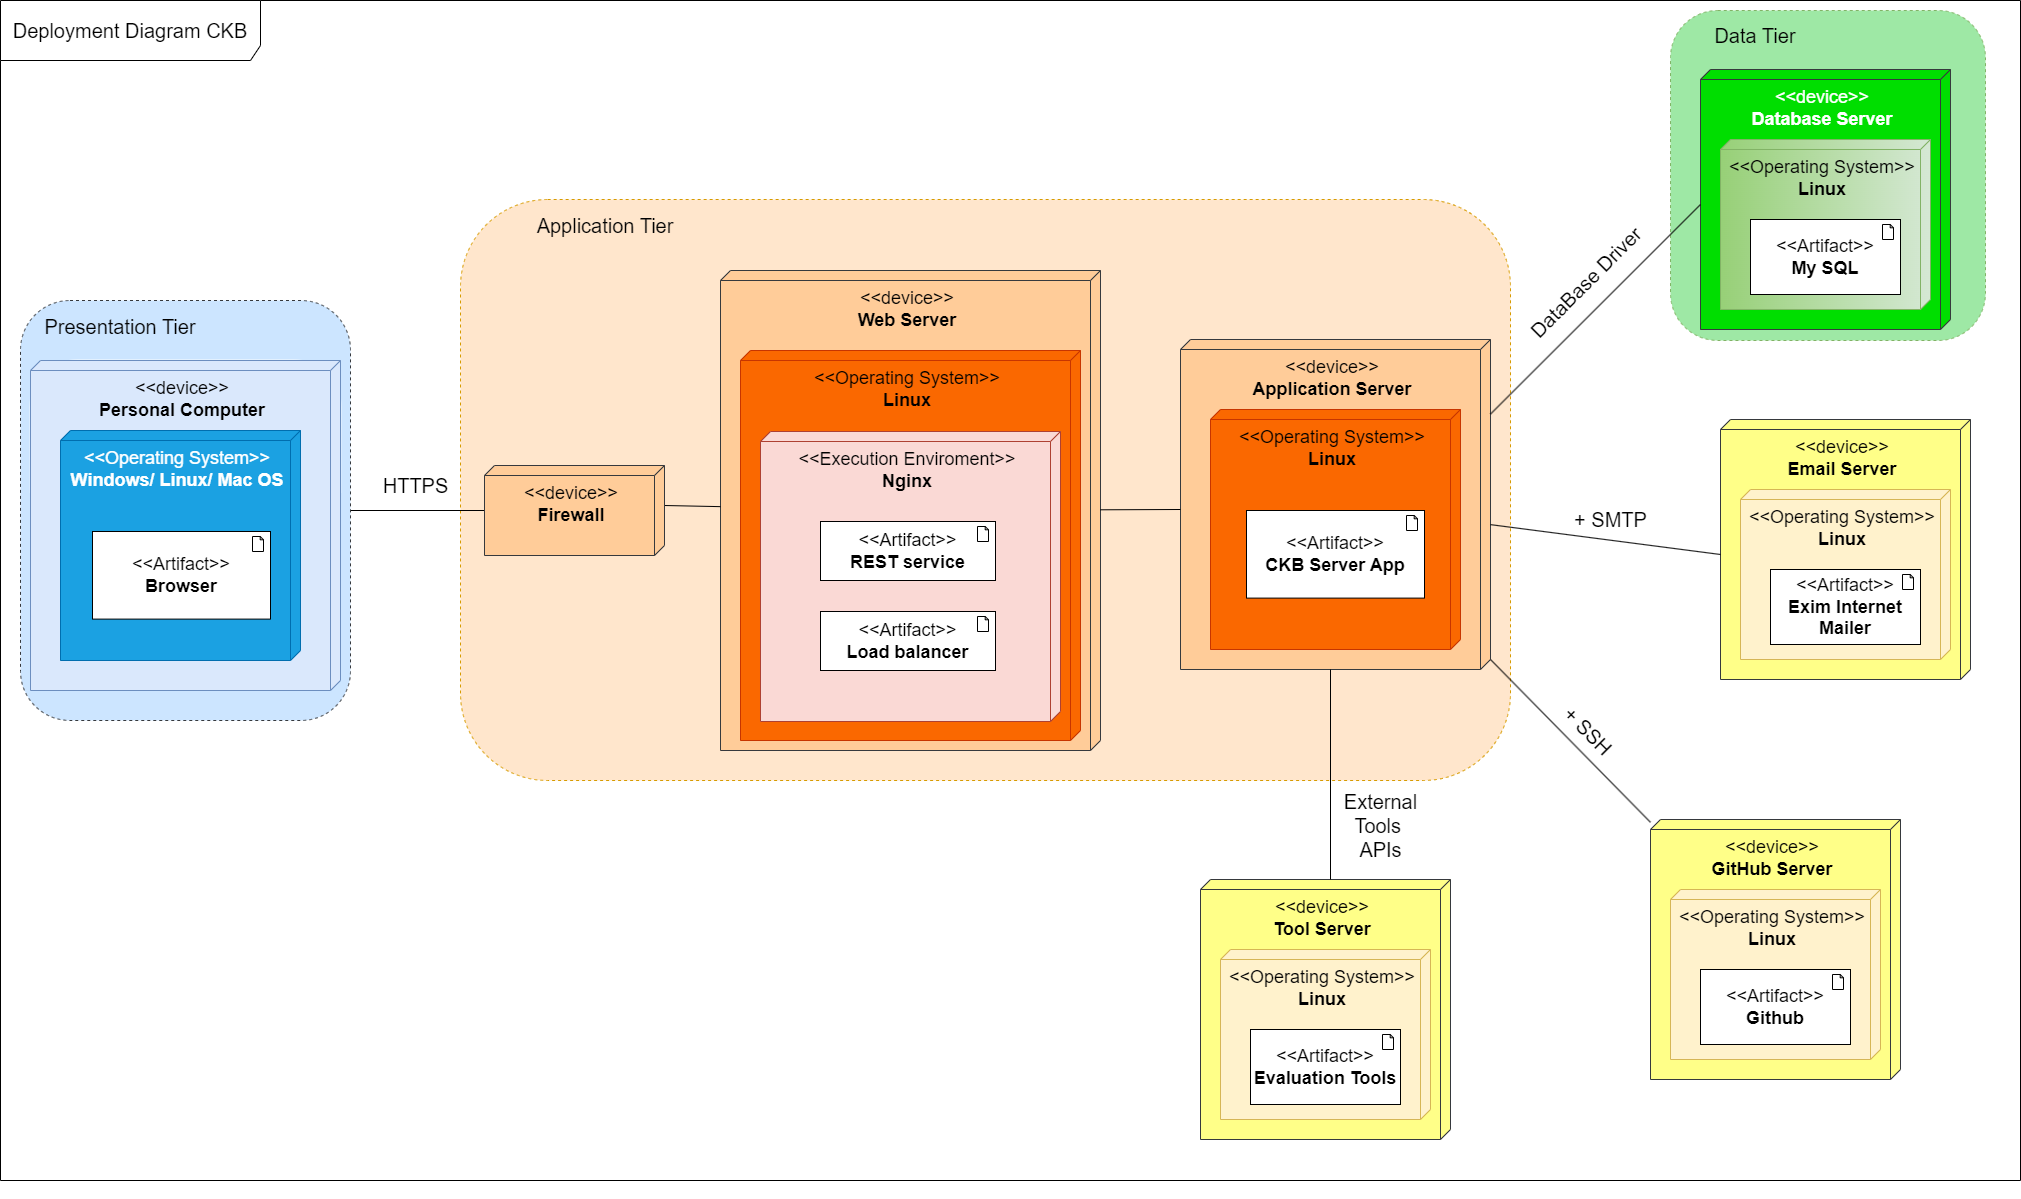
\includegraphics[width=1\linewidth]{CD_DD/DeploymentDiagram.png}
        \caption{Deployment Diagram.}
        \label{fig:Deployment_Diagram}%
    \end{center}
\end{figure}

\paragraph{Personal Computer:}
STs and EDs can access to the system by using any type of personal computer through their favorite web browser. The browser will communicate with the Web Server. Users can also use every device that allows them to search on a web browser, such as mobile phone, tablet, ecc.

\paragraph{Web Server:}
The Web Server provides access to the Application Server’s service to all the User that reaches the system through a web browser. In particular, the Web Server does not execute any business logic, but it simply does some load balancing on the receive requests from the client to the various Application Servers, in order to handle large User traffic.\\
It also provides to the client's browsers the HTML, JSON, Javascript and CSS files for making the rendering of the pages.

\paragraph{Firewall:}
It provides a way to limit the attack surface of any potential intruder by providing strict access rules.

\paragraph{Application Server:}
The application server contains the business logic of the entire system. Moreover, it communicates to the client through HTTPS protocol managed by the Web Server. The various requests coming from the Web Server are routed to the corresponding module thanks to the Dashboard Manager.\\
Furthermore, it communicates to the Database Server through the model gateway. This node is replicated in order to handle large user traffic.

\paragraph{Database Server:}
All the Data about Tournaments, Battles, Users, Groups and Badges are stored into the Database Server and managed by MySQL.\\
The various Application Servers can retrieve information on this node through the model module and the database driver.

\paragraph{Email Server:}
After the registration, Users have to click on the link sent by eMail to confirm their profile. The Application Server, immediately after the registration, contacts the Email Server through SMTP protocol to send the confirmation eMail to the User.

\paragraph{Github Server:}
The dialogs with the Application Server node occur during the different Battle phases: when the ED creates a new Battle also a GitHub repository is created containing the code kata of the Battle and it is subsequently forked from the various STG.\\
The GitHub Server is also periodically contacted for retrieving newly committed code on the main branch of the different STGs' repositories.
For those scopes, the Application Server shall communicate with the Github Server through the SSH protocol.


\paragraph{Tool Server:}
With the External Tool APIs the Application Server can contact the Tool Server and pass to it the code retrieved from the Github Server to be tested and evaluated.

\newpage
\section{Runtime View}
\label{sec:runtime_view}%

\subsection{Log in to the system}
\begin{figure}[H]
    \begin{center}
        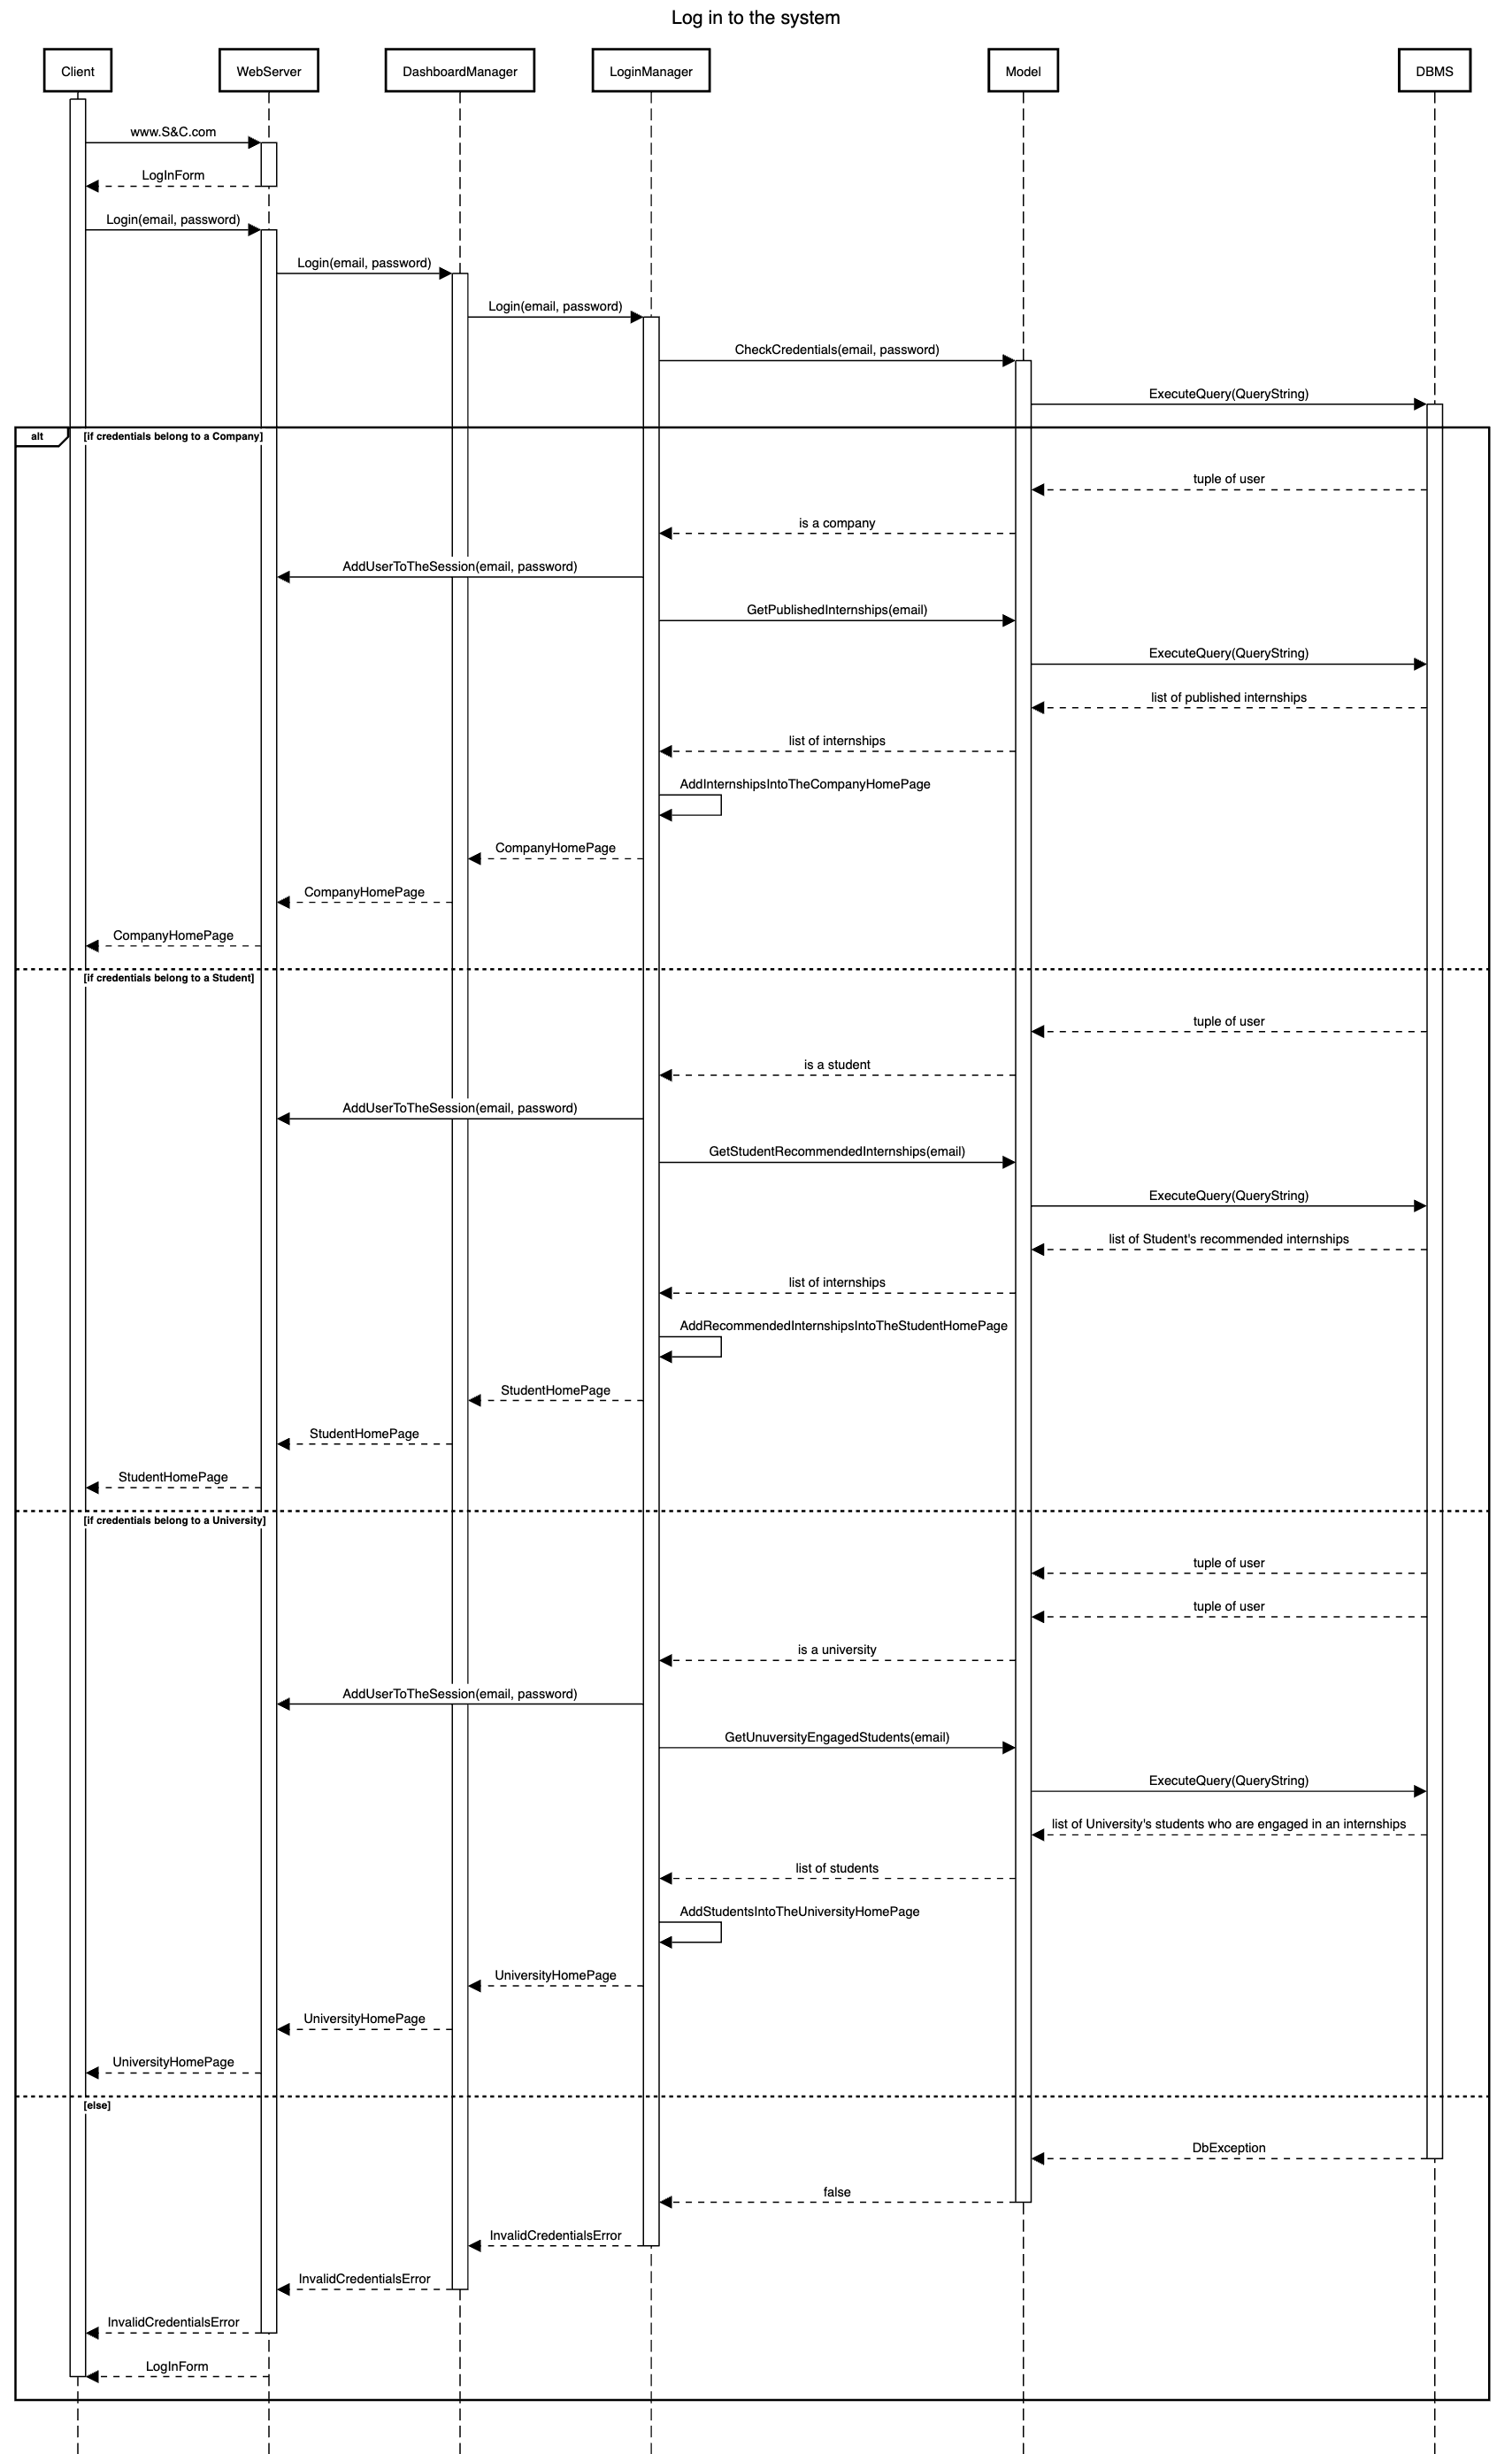
\includegraphics[width=0.8\linewidth]{DD/LaTeX/Images/RuntimeView/LogIn.png}
        \caption{Runtime view for 'Log in to the system'.}
        \label{fig:runtime_LogIn}%
    \end{center}
\end{figure}

DESCRIPTION


\subsection{Log out from the system}
\begin{figure}[H]
    \begin{center}
        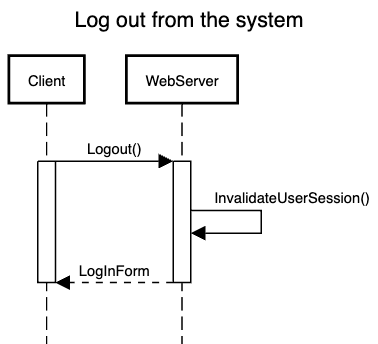
\includegraphics[width=0.8\linewidth]{DD/LaTeX/Images/RuntimeView/LogOut.png}
        \caption{Runtime view for 'Log out from the system'.}
        \label{fig:runtime_LogOu}%
    \end{center}
\end{figure}

DESCRIPTION


\subsection{Register an account to S\&C}
\begin{figure}[H]
    \begin{center}
        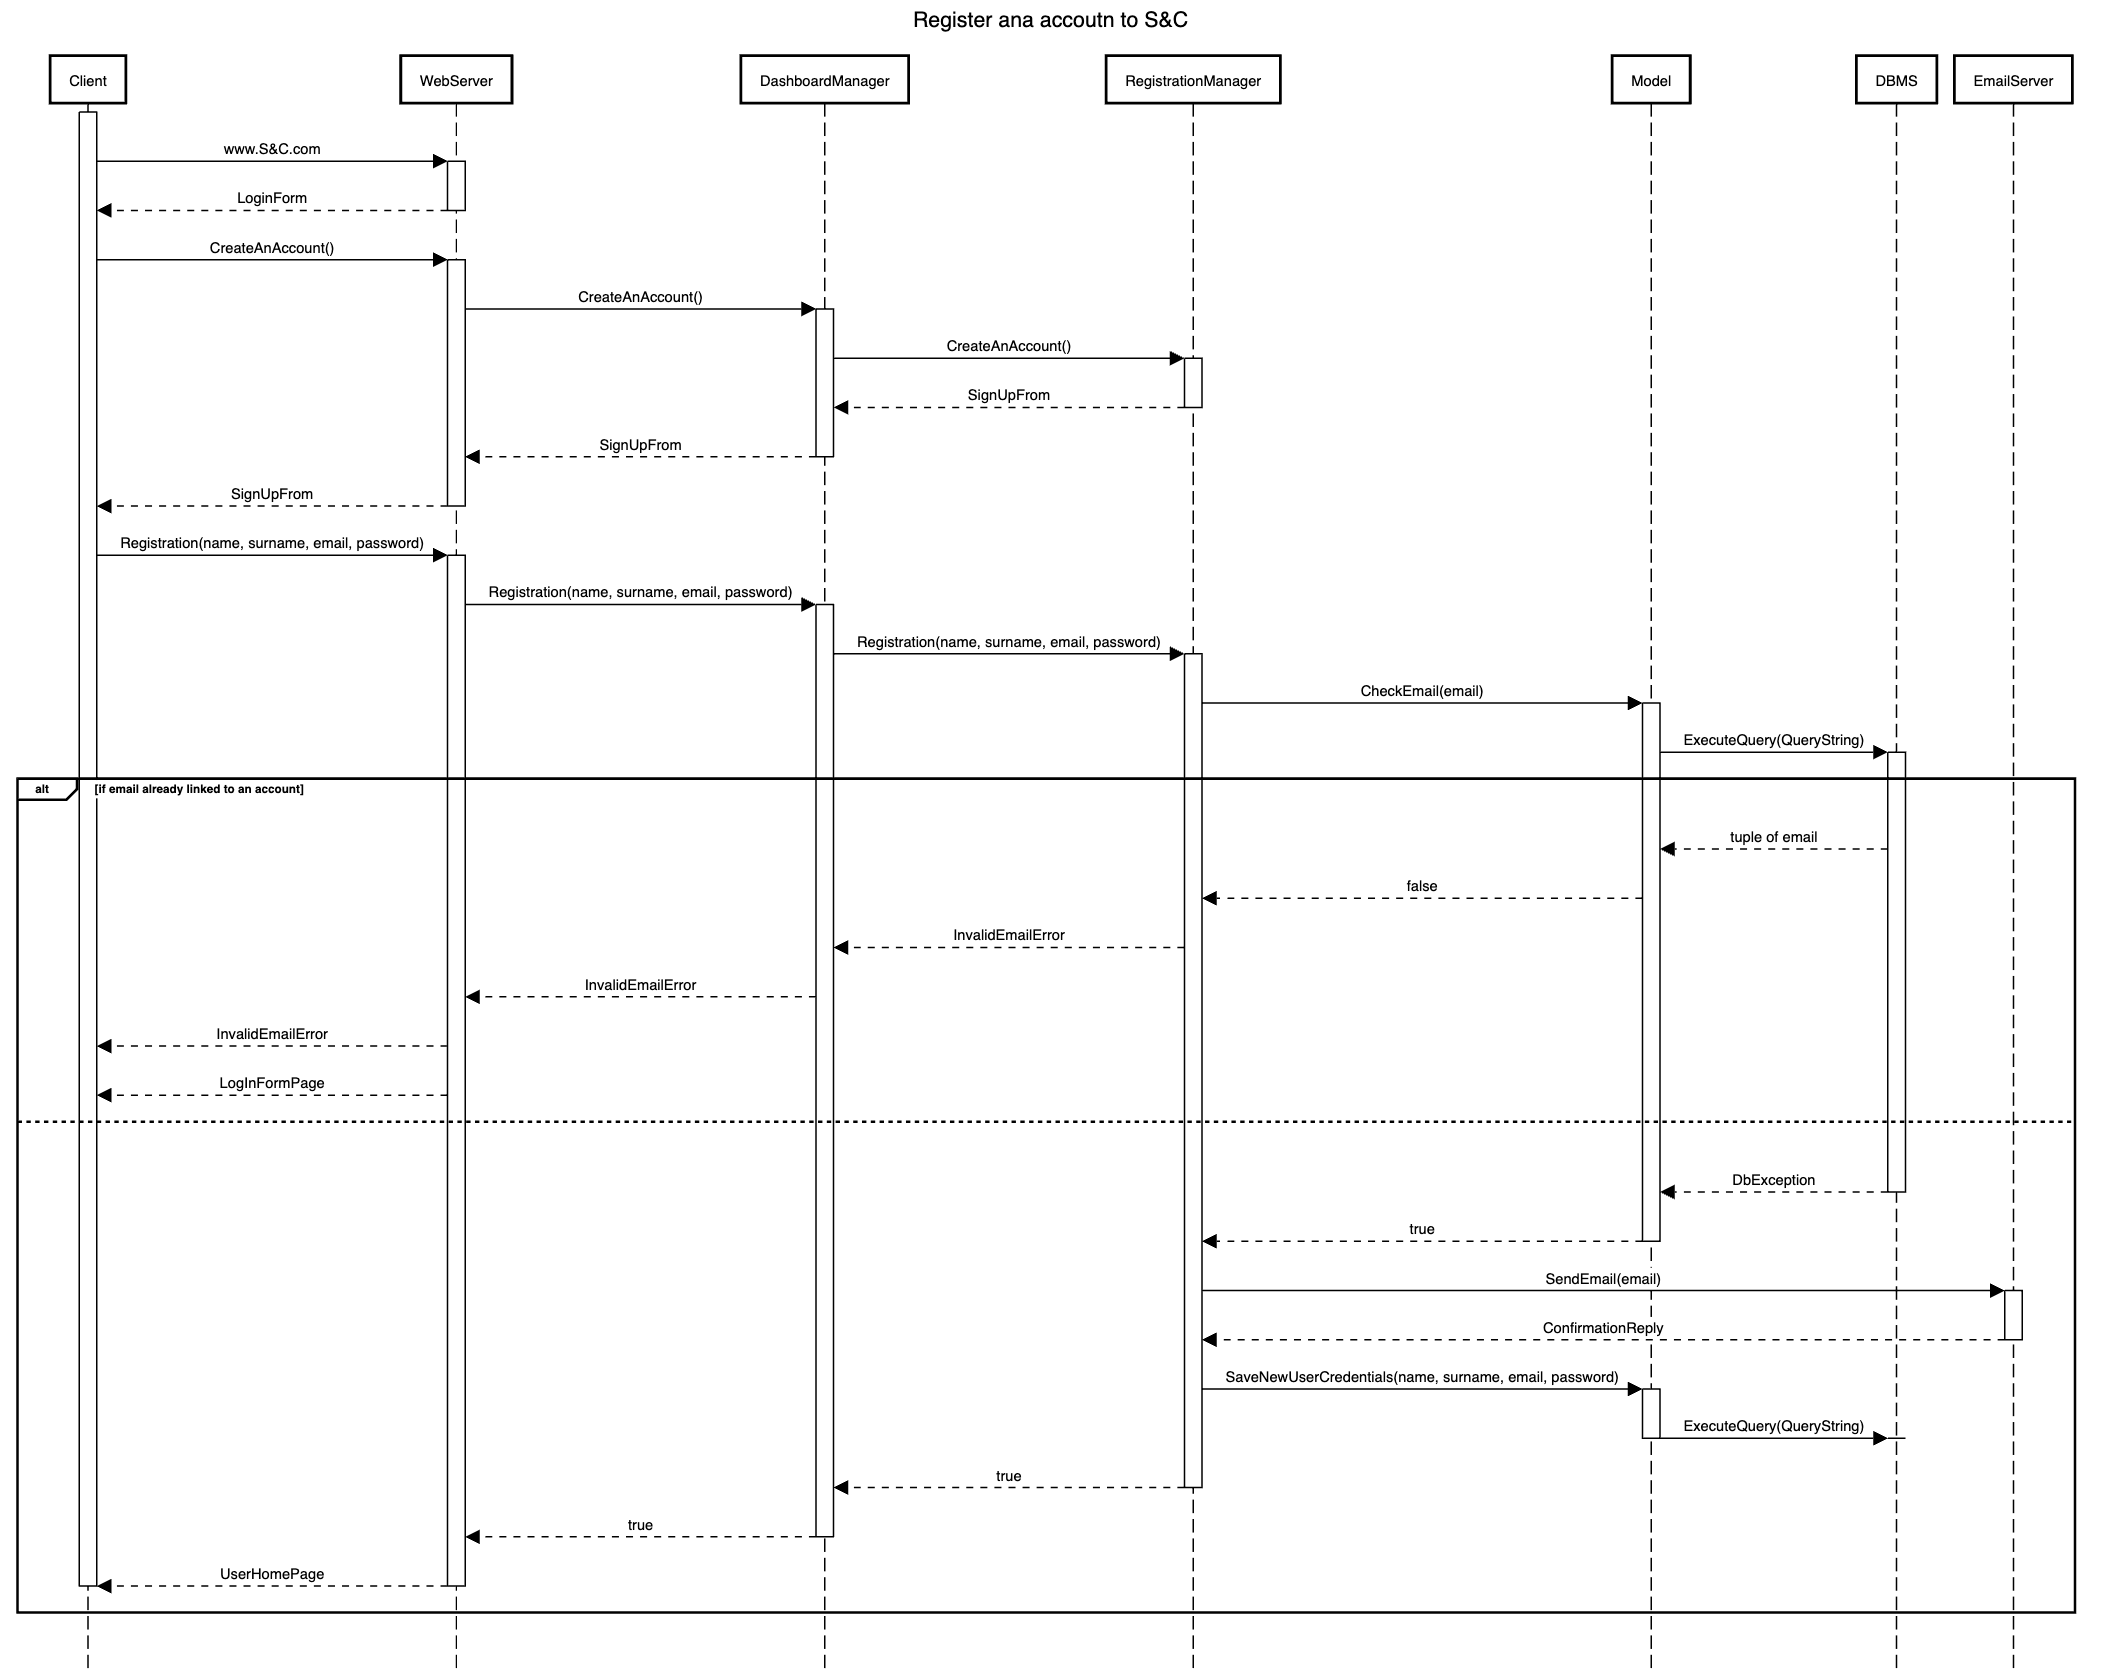
\includegraphics[width=0.8\linewidth]{DD/LaTeX/Images/RuntimeView/SignUp.png}
        \caption{Runtime view for 'Register an account to S\&C'.}
        \label{fig:runtime_SignUp}%
    \end{center}
\end{figure}

DESCRIPTION


\subsection{View and update their profile}
\begin{figure}[H]
    \begin{center}
        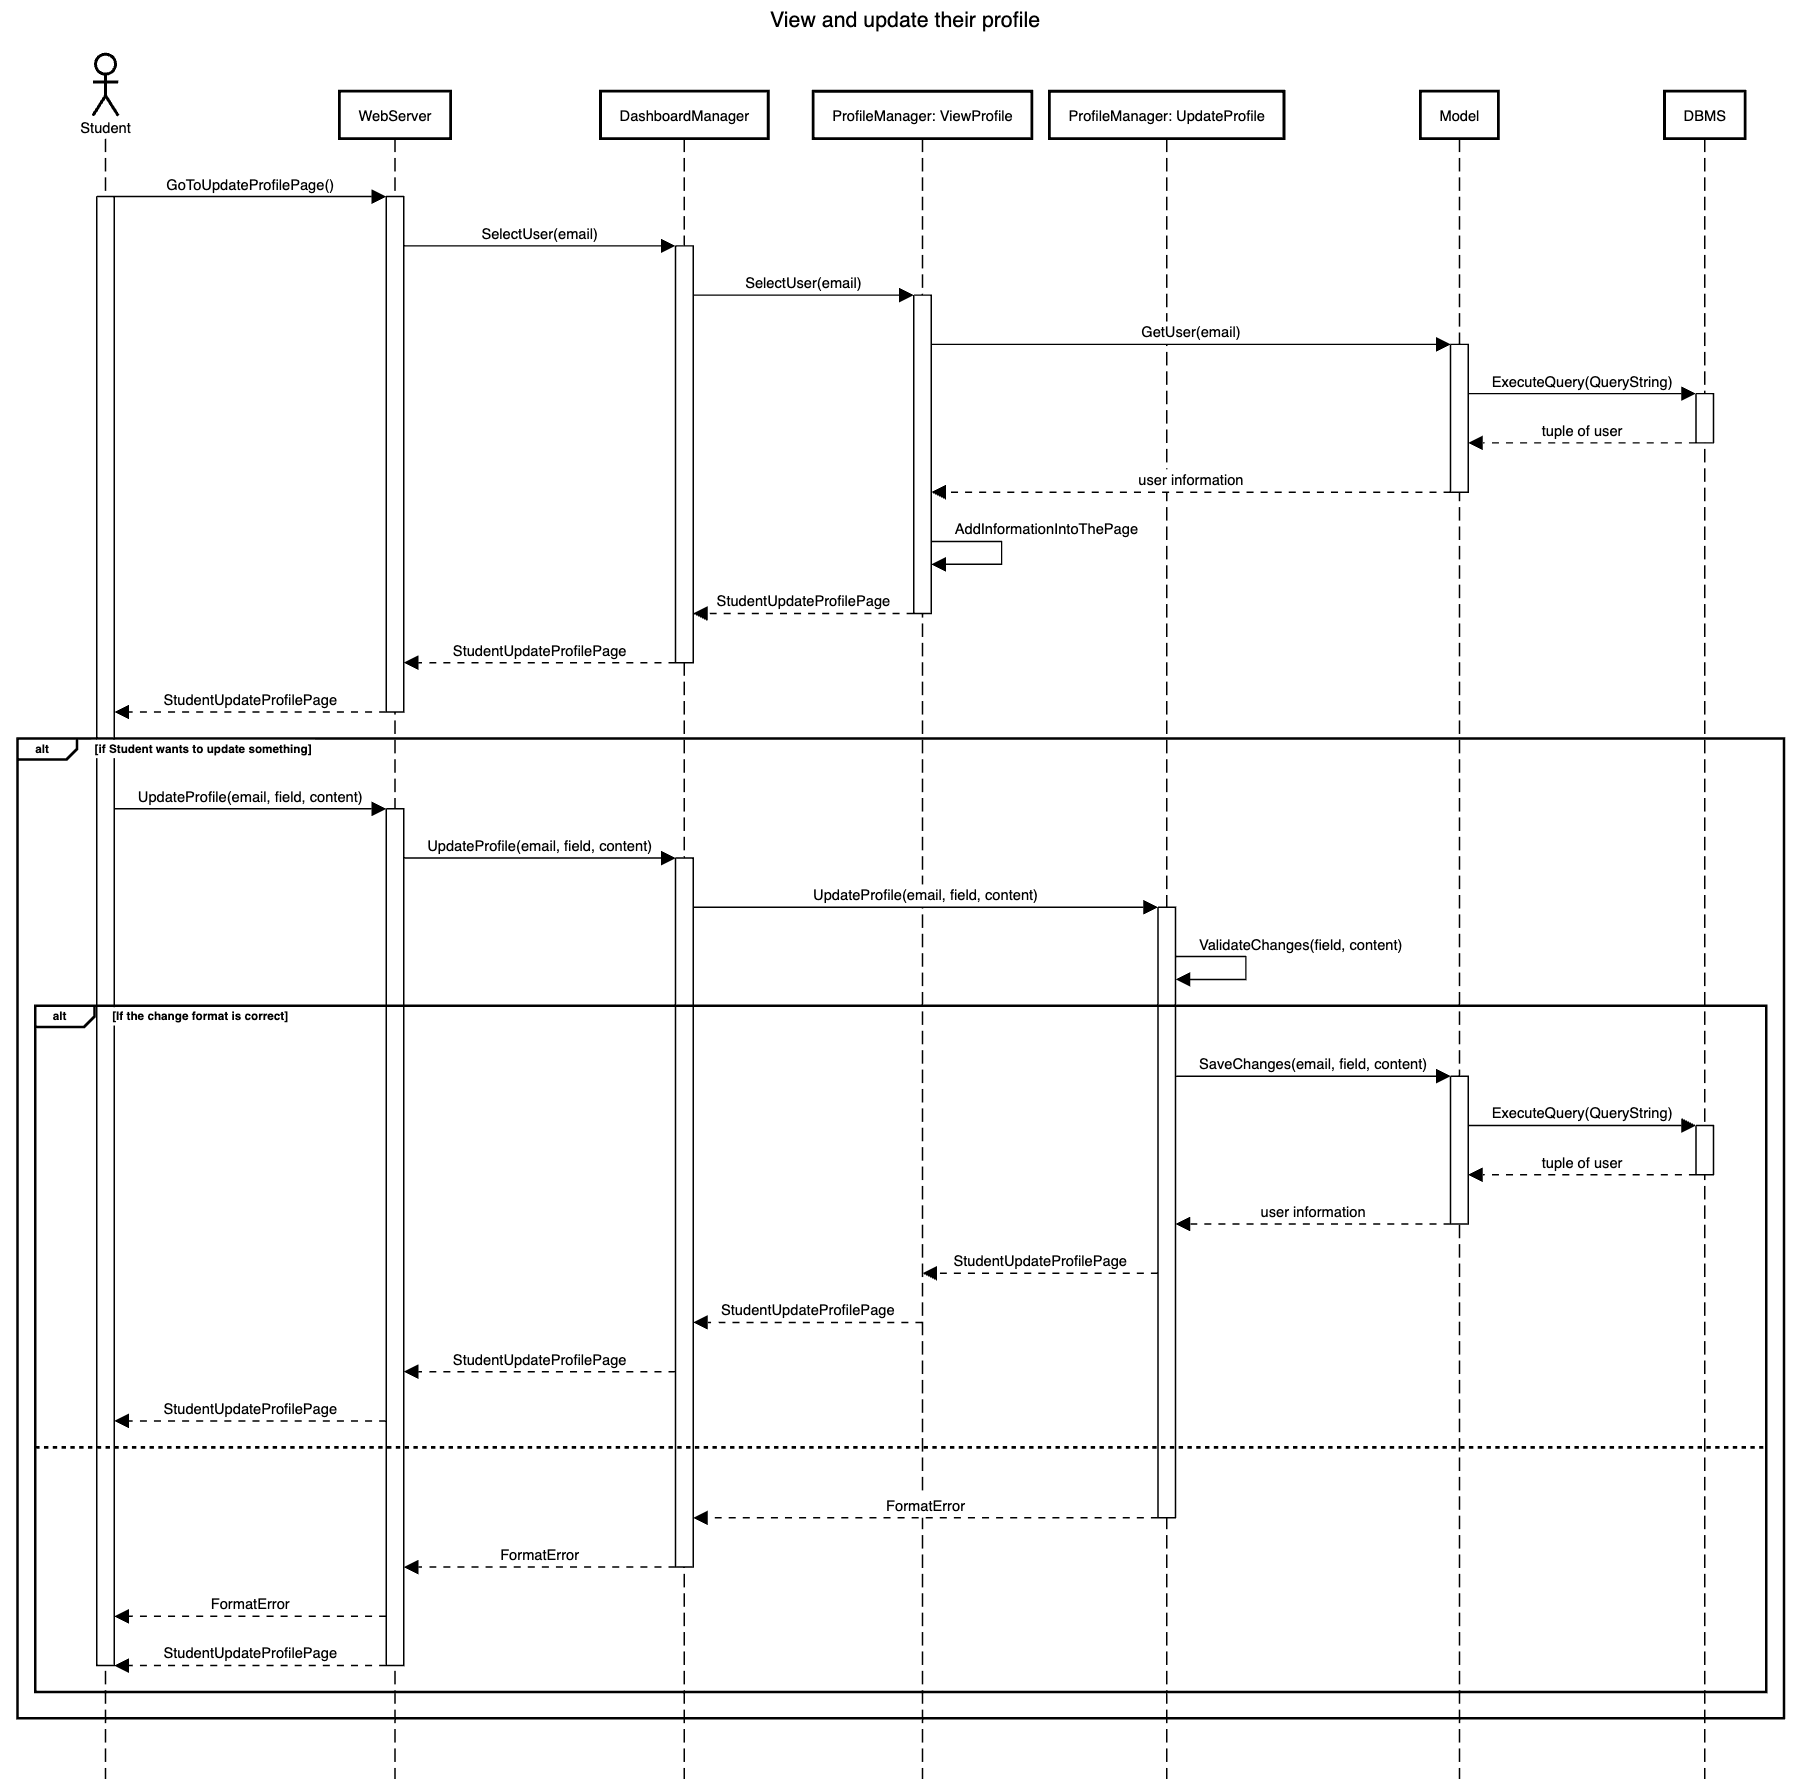
\includegraphics[width=0.8\linewidth]{DD/LaTeX/Images/RuntimeView/ViewAndUpdateTheirProfile.png}
        \caption{Runtime view for 'View and update their profile'.}
        \label{fig:runtime_ViewAndUpdateTheirProfile}%
    \end{center}
\end{figure}

DESCRIPTION


\subsection{Search for internships}
\begin{figure}[H]
    \begin{center}
        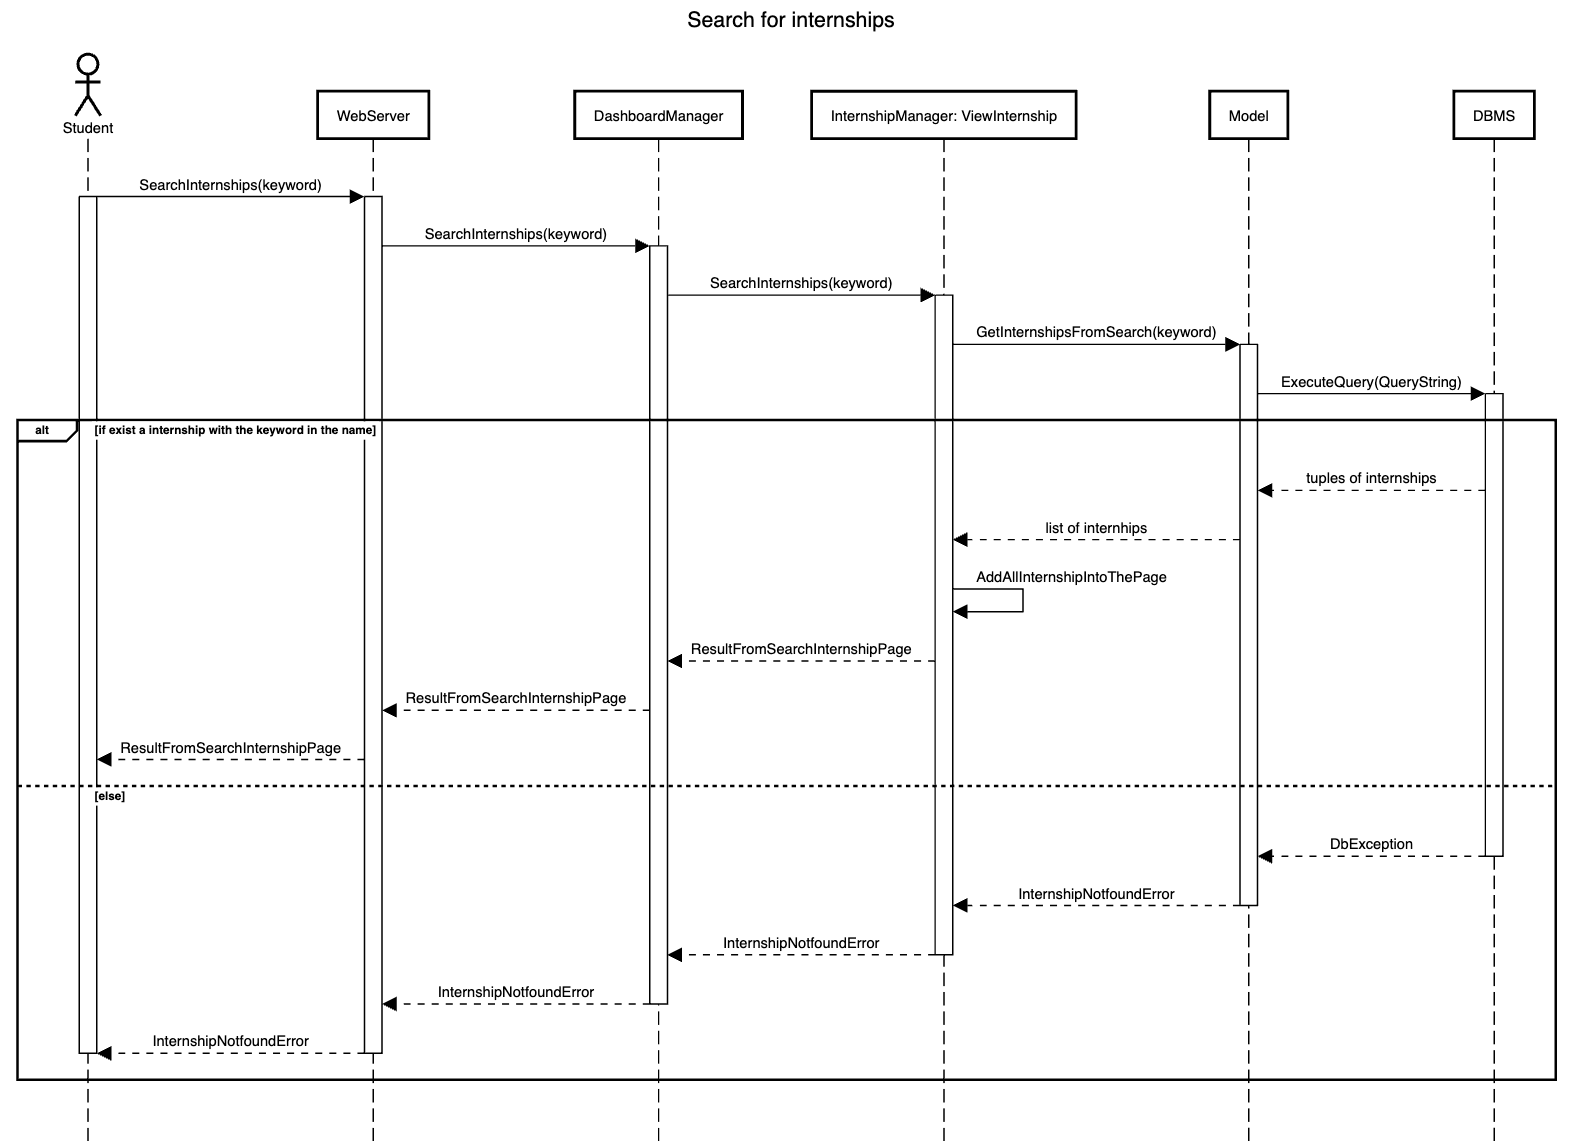
\includegraphics[width=0.8\linewidth]{DD/LaTeX/Images/RuntimeView/SearchInternship.png}
        \caption{Runtime view for 'Search for internships'.}
        \label{fig:runtime_SearchInternship}%
    \end{center}
\end{figure}

DESCRIPTION


\subsection{Apply for an internship}
\begin{figure}[H]
    \begin{center}
        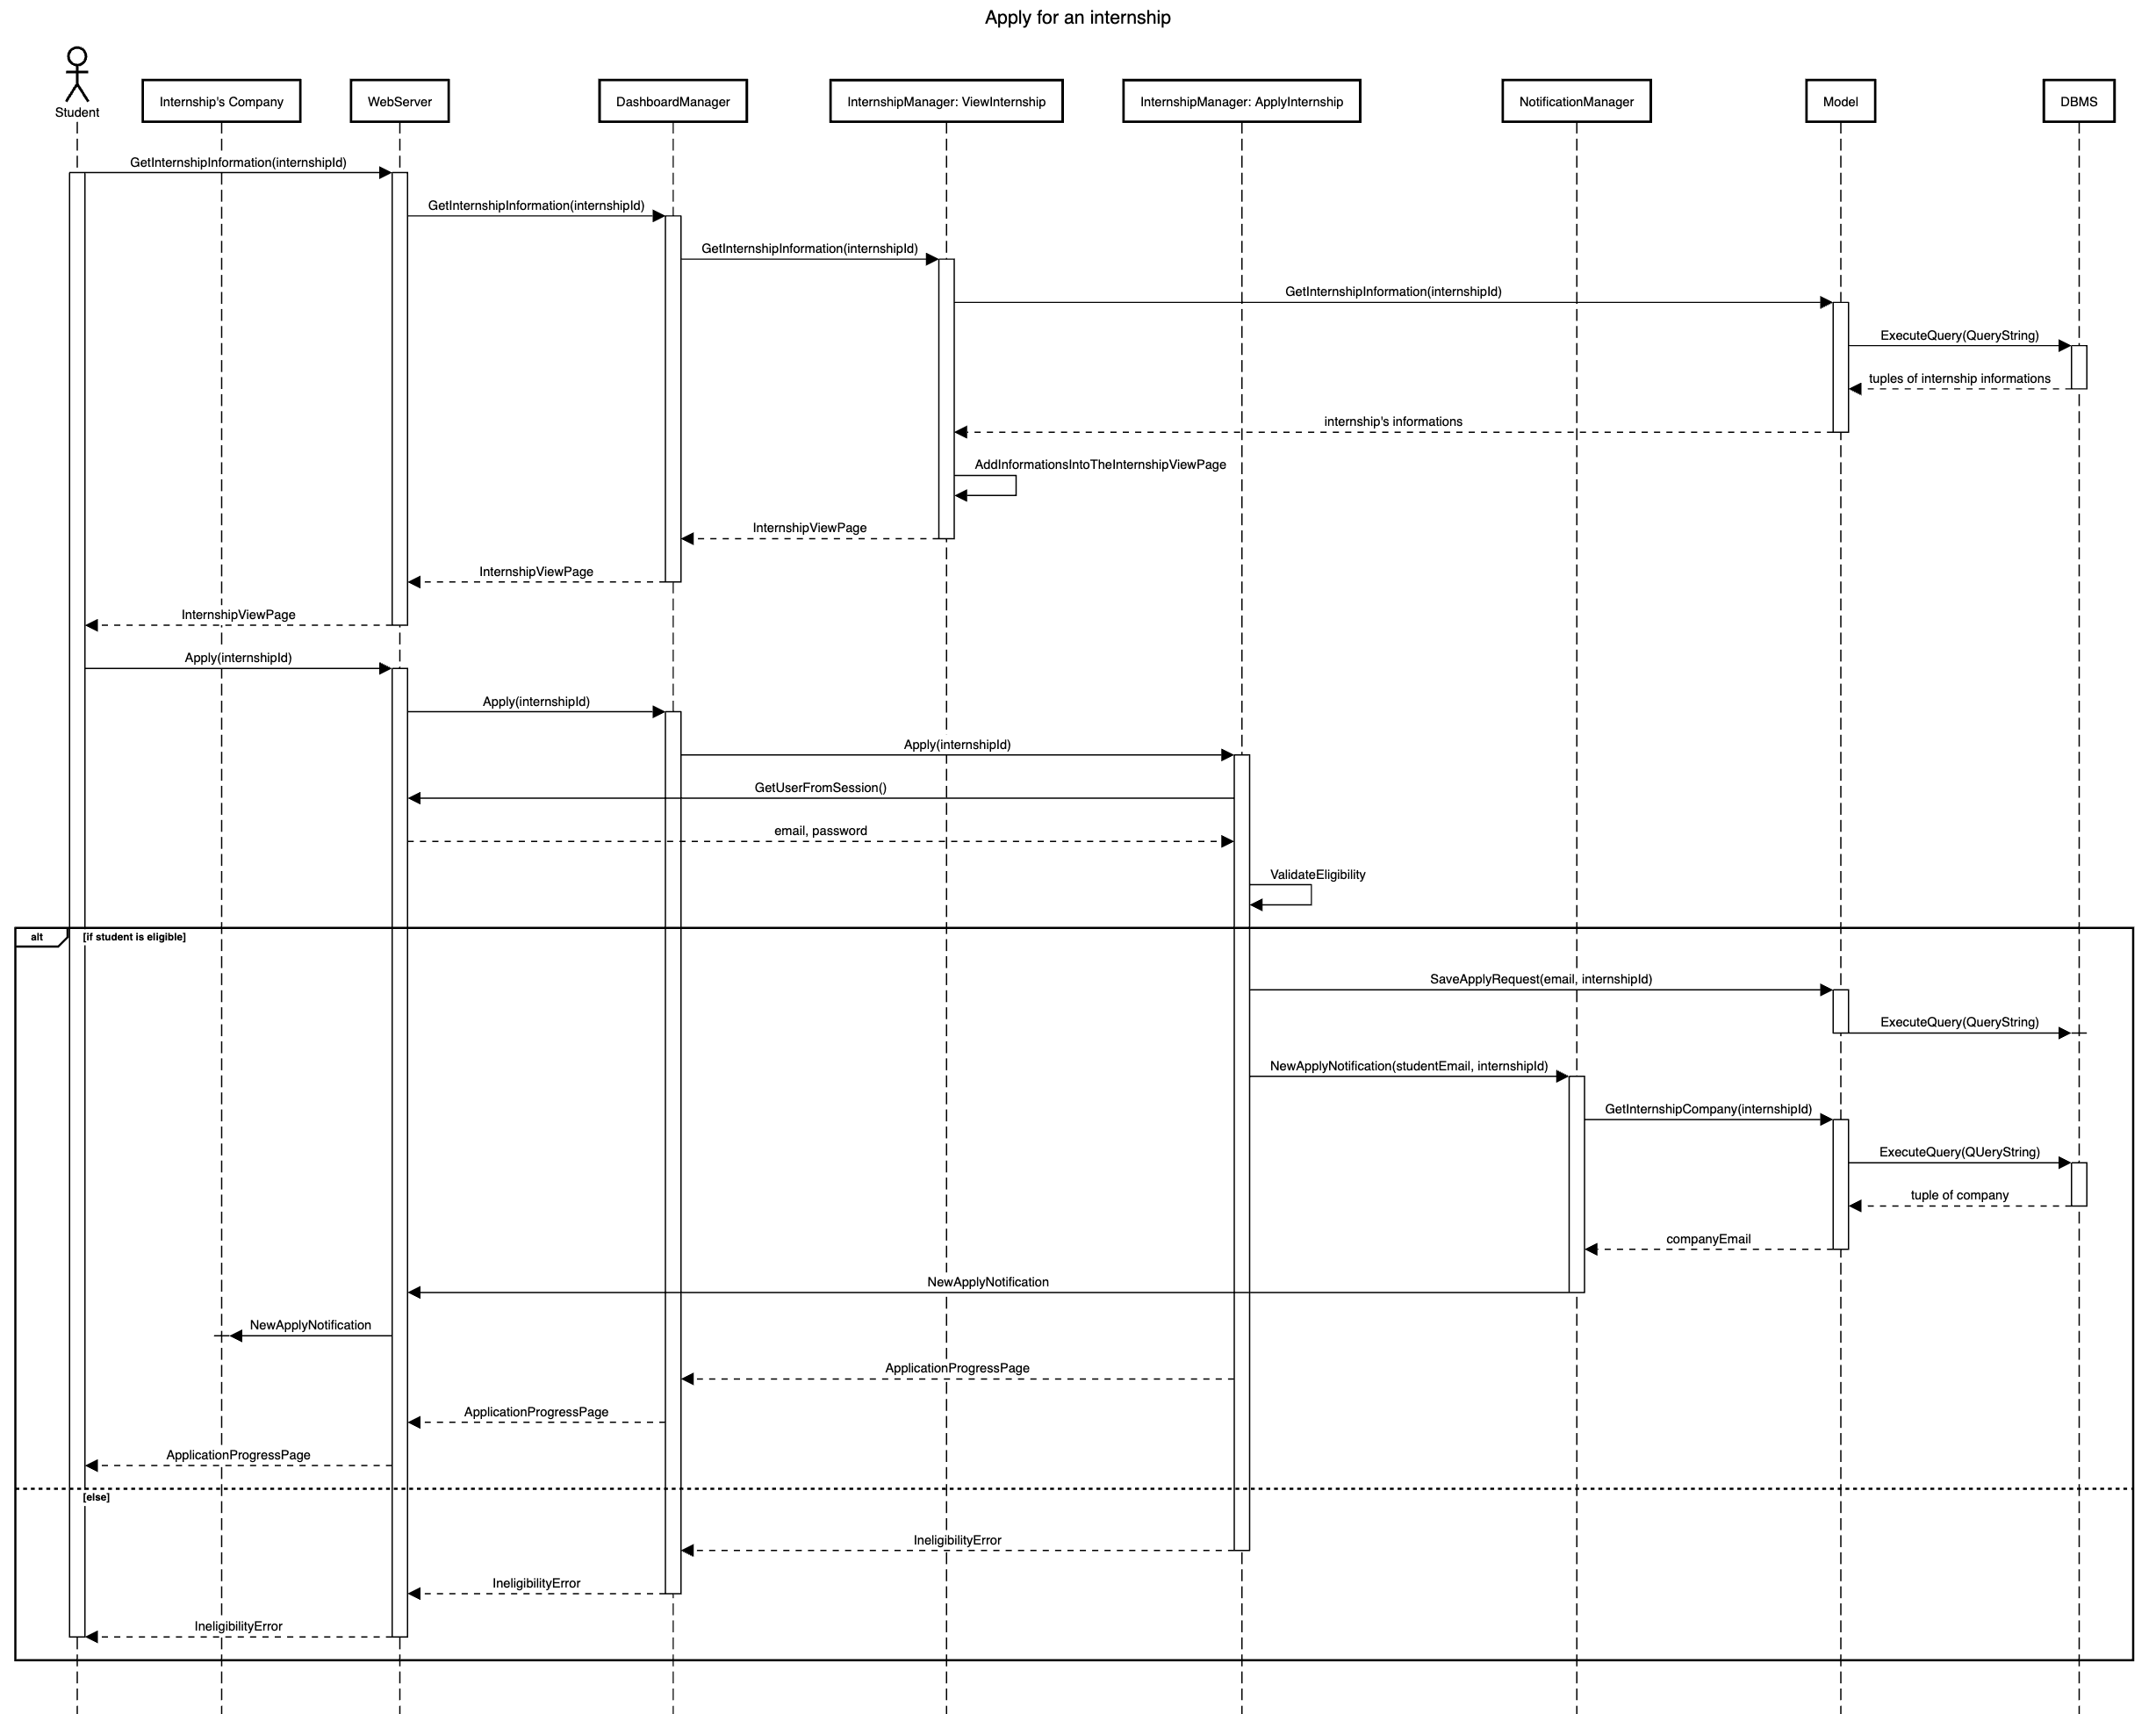
\includegraphics[width=0.8\linewidth]{DD/LaTeX/Images/RuntimeView/ApplyInternship.png}
        \caption{Runtime view for 'Apply for an internship'.}
        \label{fig:runtime_ApplyInternship}%
    \end{center}
\end{figure}
DESCRIPTION


\subsection{Monitor the status of their applications}
\begin{figure}[H]
    \begin{center}
        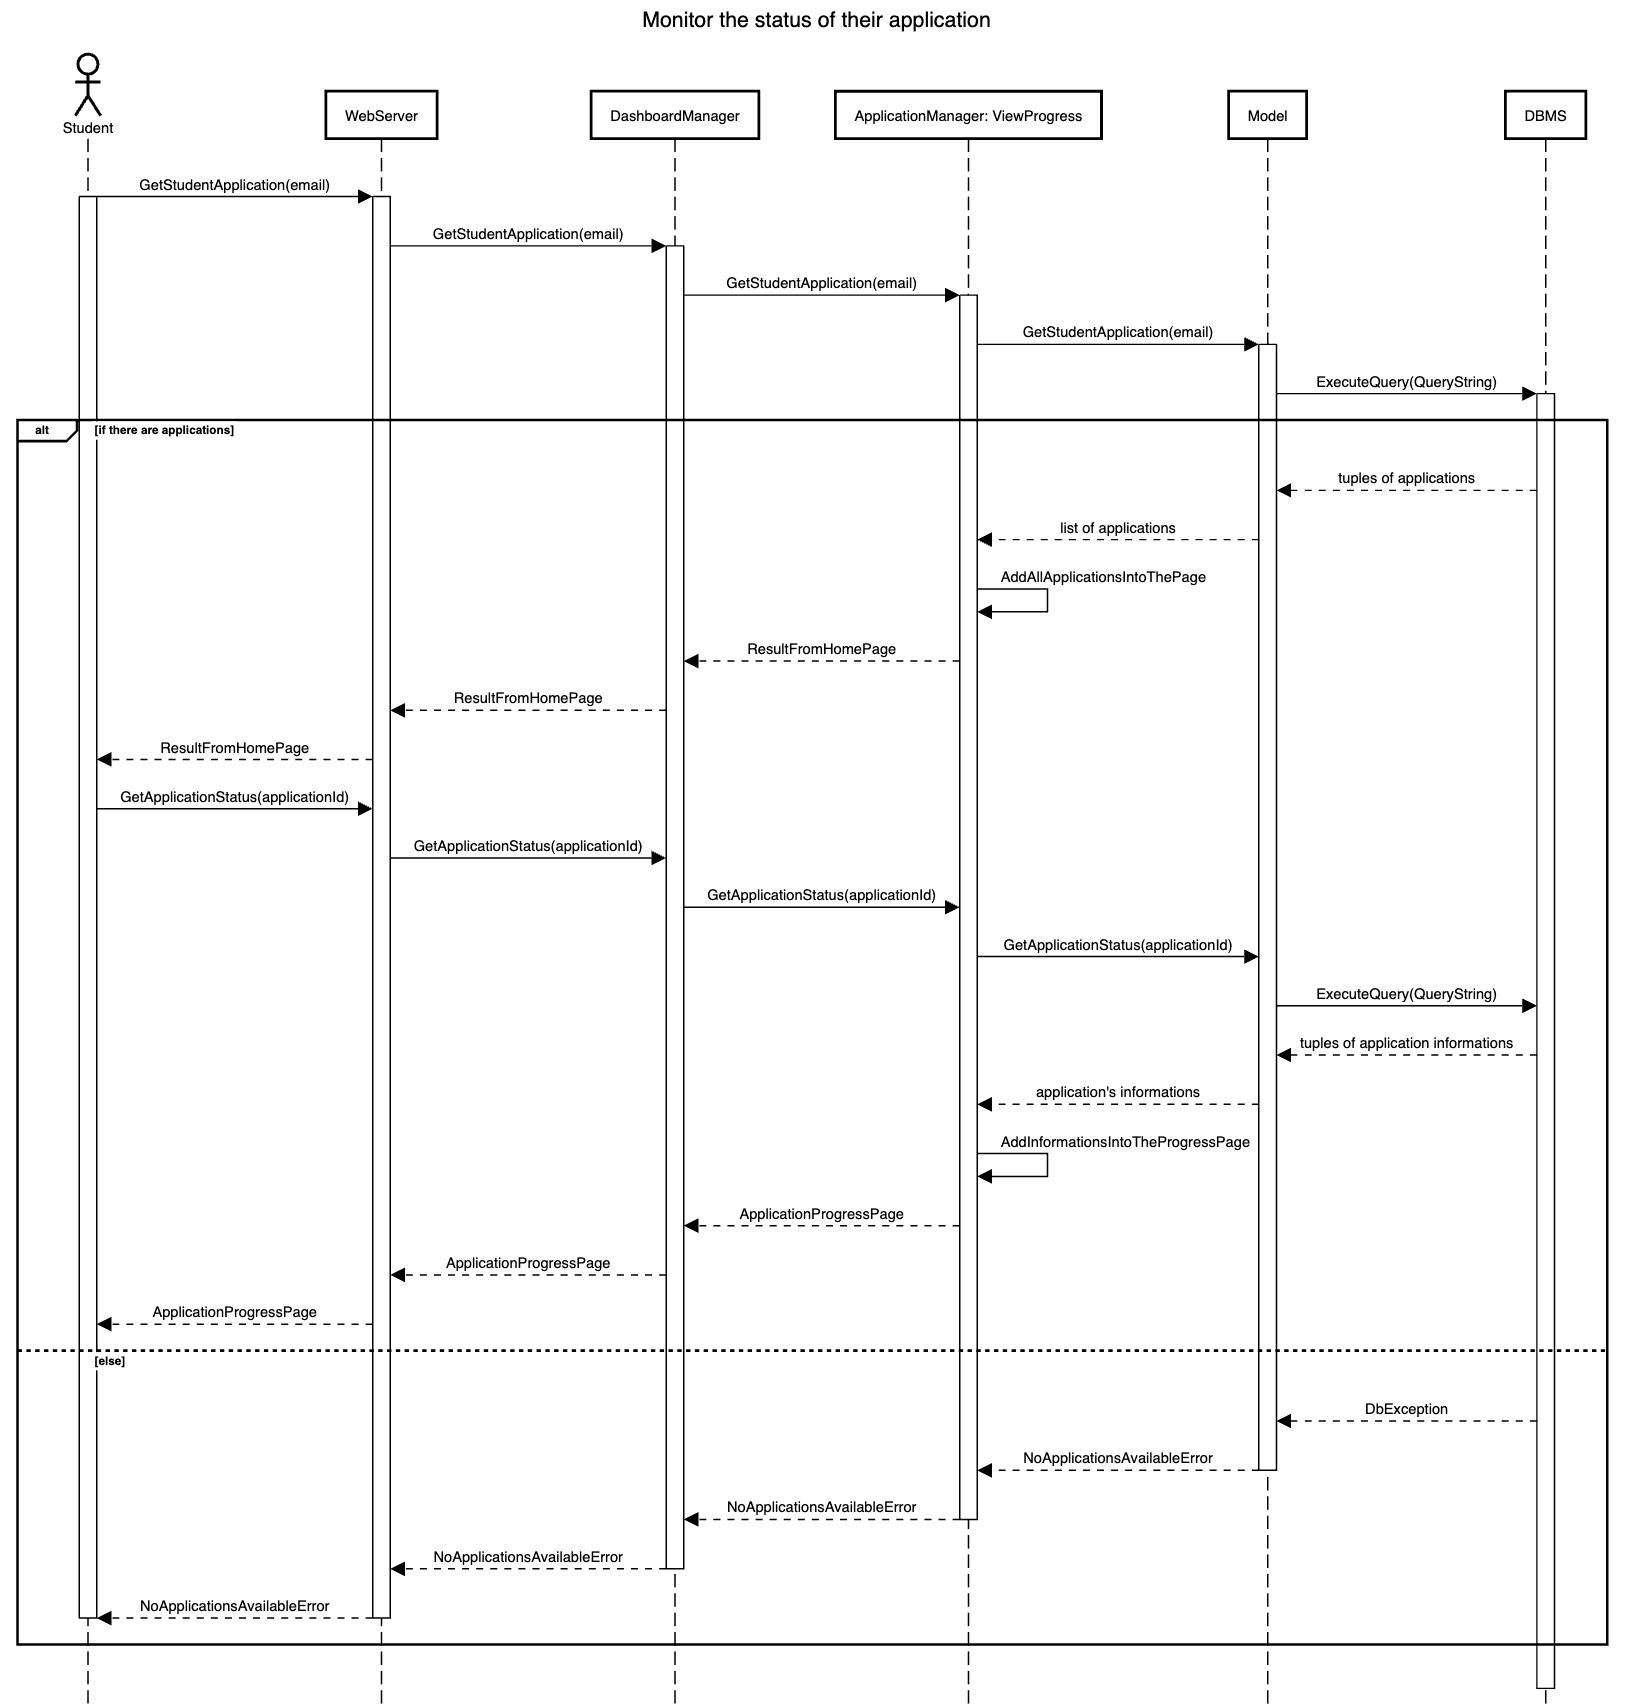
\includegraphics[width=0.8\linewidth]{DD/LaTeX/Images/RuntimeView/MonitorStatusApplication.png}
        \caption{Runtime view for 'Monitor the status of their applications'.}
        \label{fig:runtime_MonitorStatusApplication}%
    \end{center}
\end{figure}

DESCRIPTION


\subsection{Accept or reject internship offers}
\begin{figure}[H]
    \begin{center}
        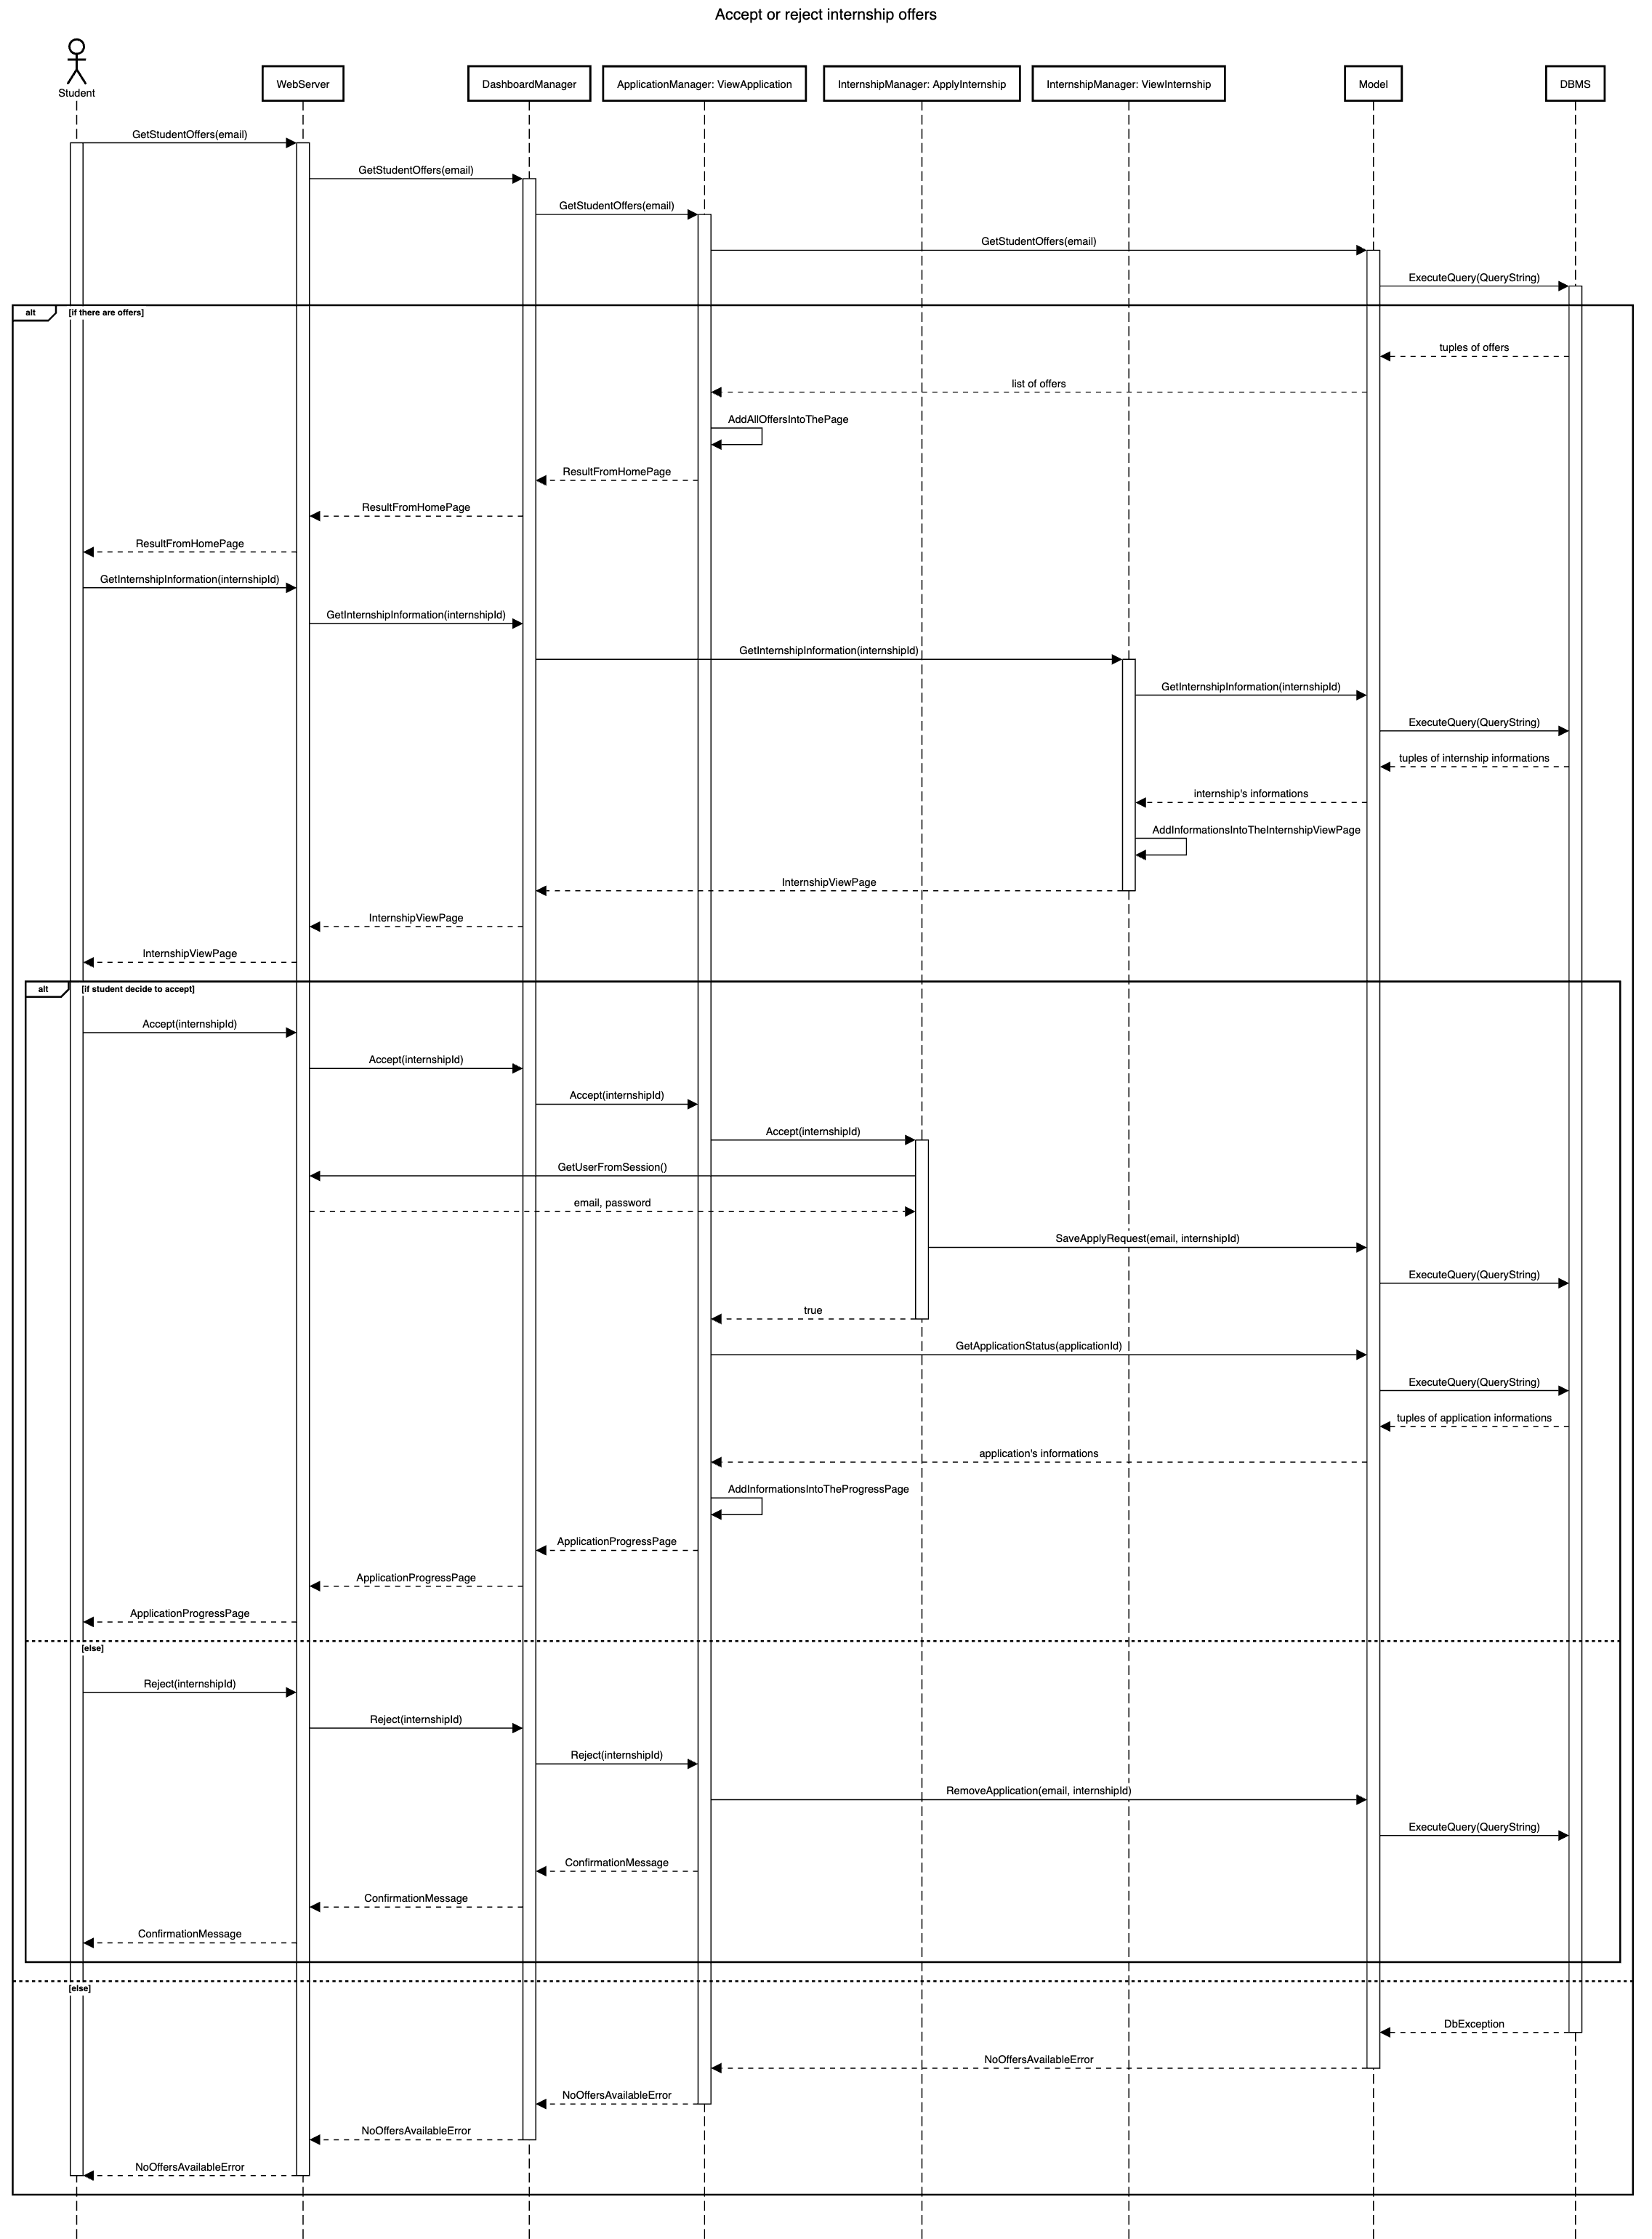
\includegraphics[width=0.8\linewidth]{DD/LaTeX/Images/RuntimeView/EvaluationInternshipOffers.png}
        \caption{Runtime view for 'Accept or reject internship offers'.}
        \label{fig:runtime_EvaluationInternshipOffers}%
    \end{center}
\end{figure}

DESCRIPTION


\subsection{Complete questionnaires from companies}
\begin{figure}[H]
    \begin{center}
        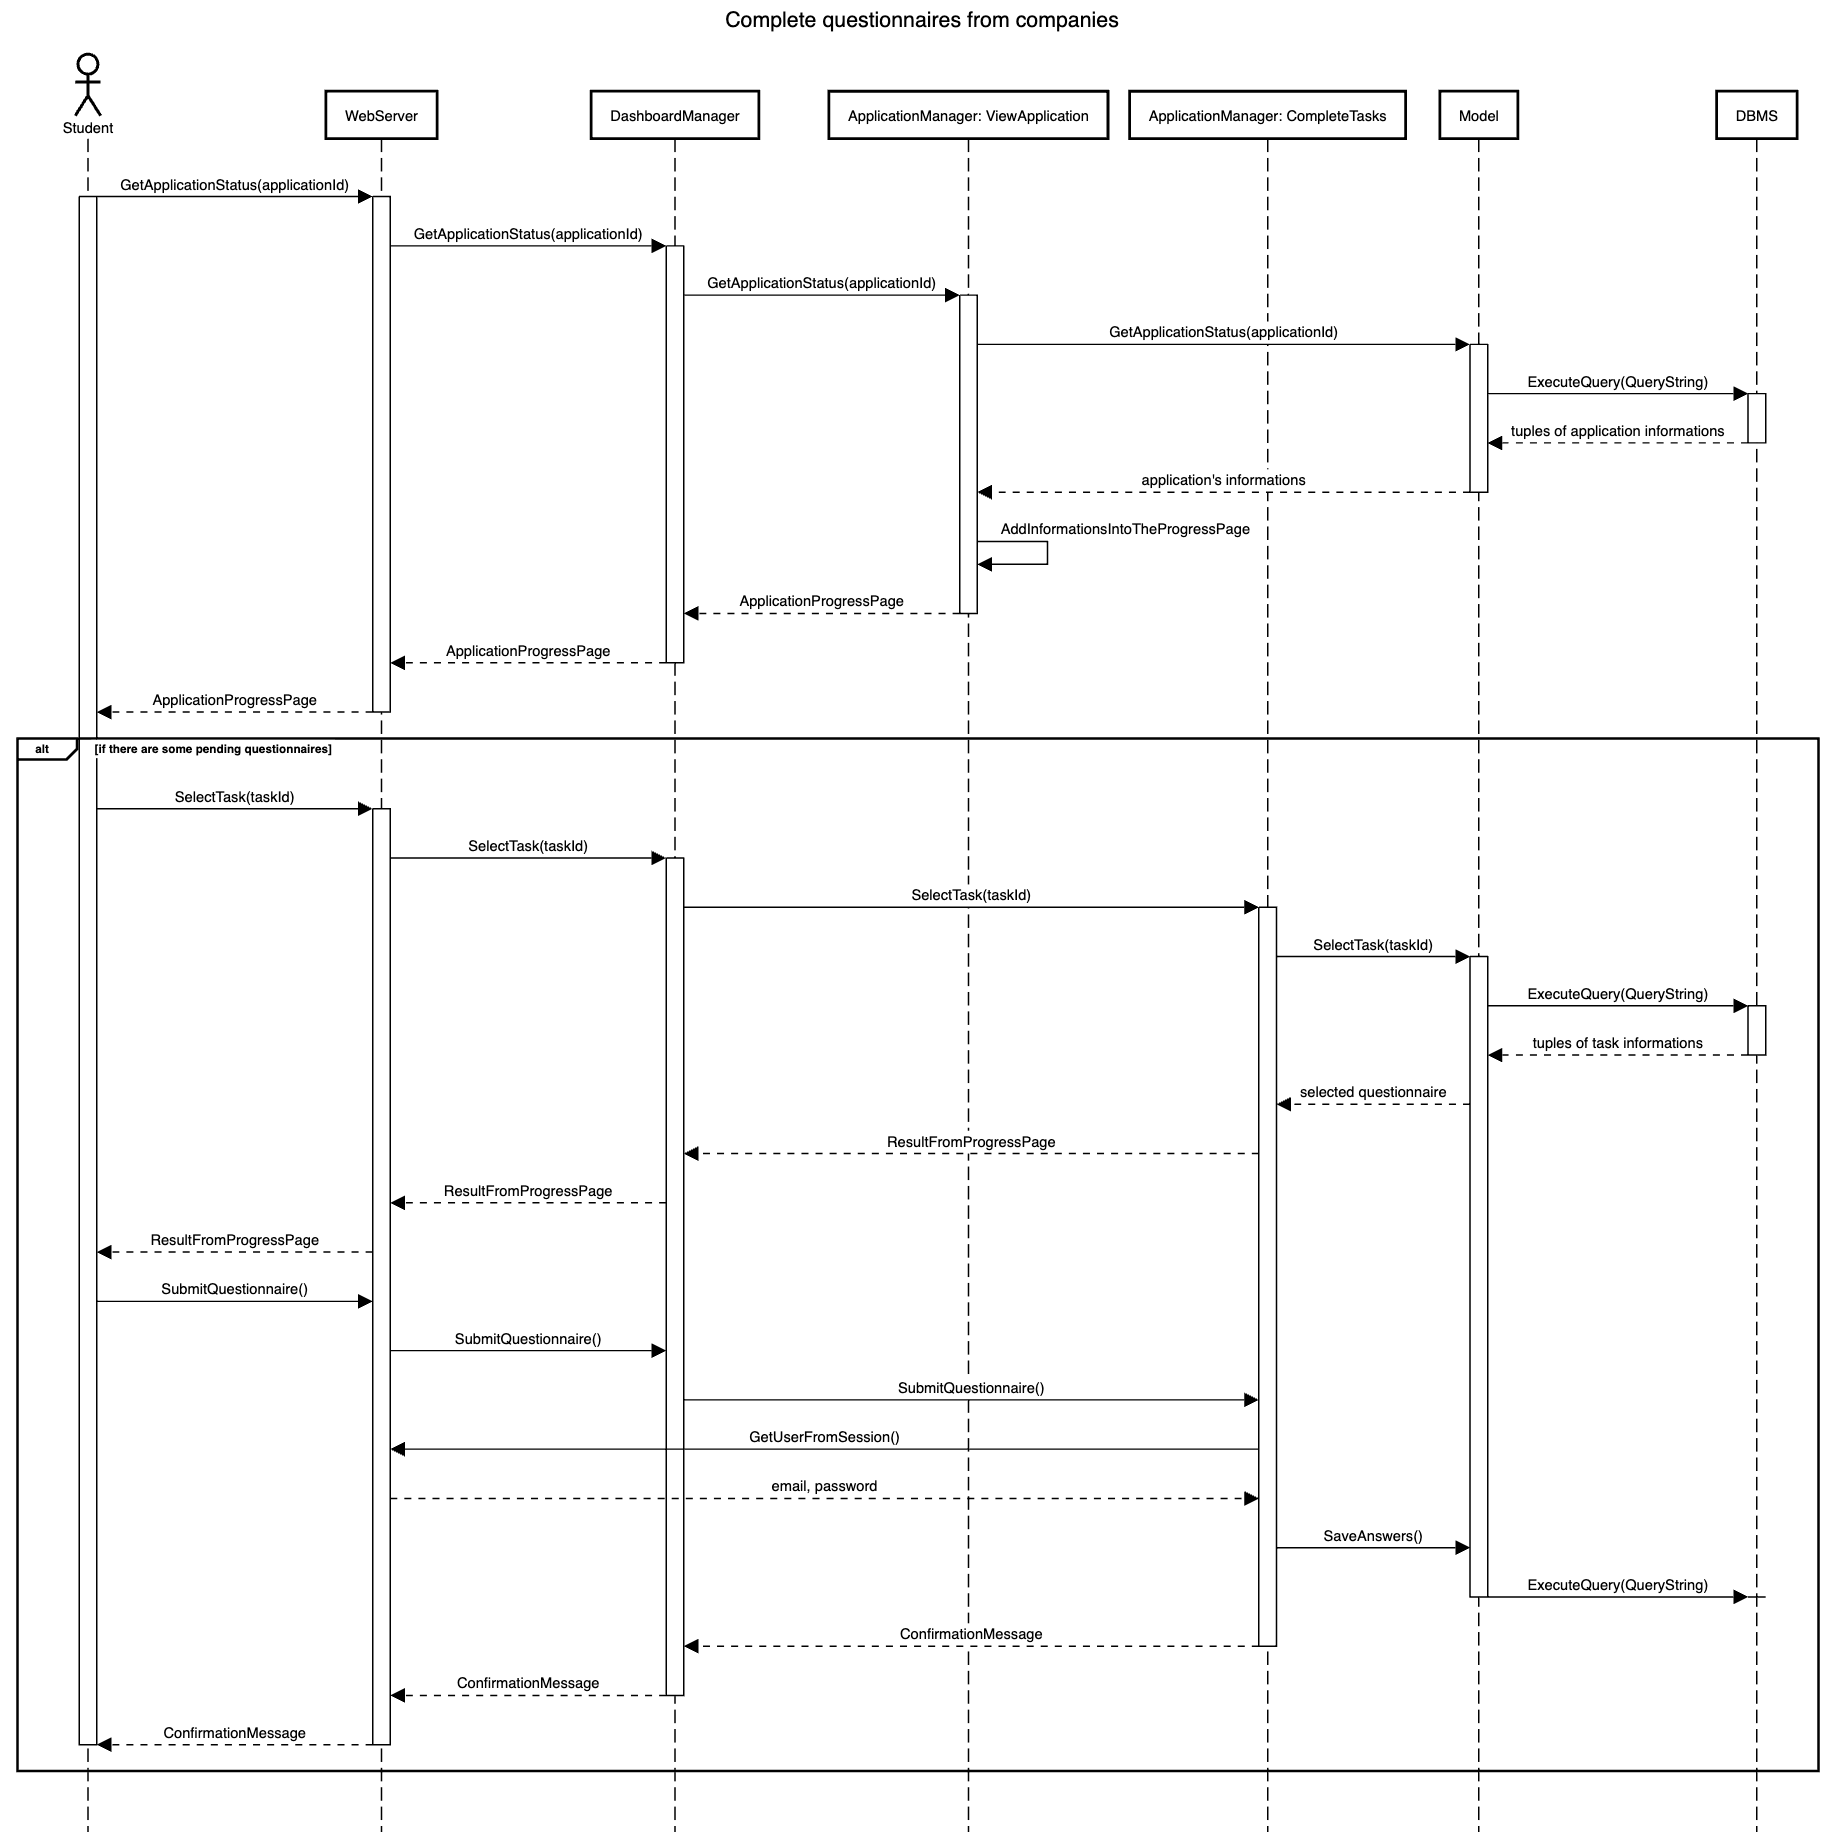
\includegraphics[width=0.8\linewidth]{DD/LaTeX/Images/RuntimeView/CompleteQuestionnaires.png}
        \caption{Runtime view for 'Complete questionnaires from companies'.}
        \label{fig:runtime_CompleteQuestionnaires}%
    \end{center}
\end{figure}

DESCRIPTION


\subsection{Provide feedback on completed internships}
\begin{figure}[H]
    \begin{center}
        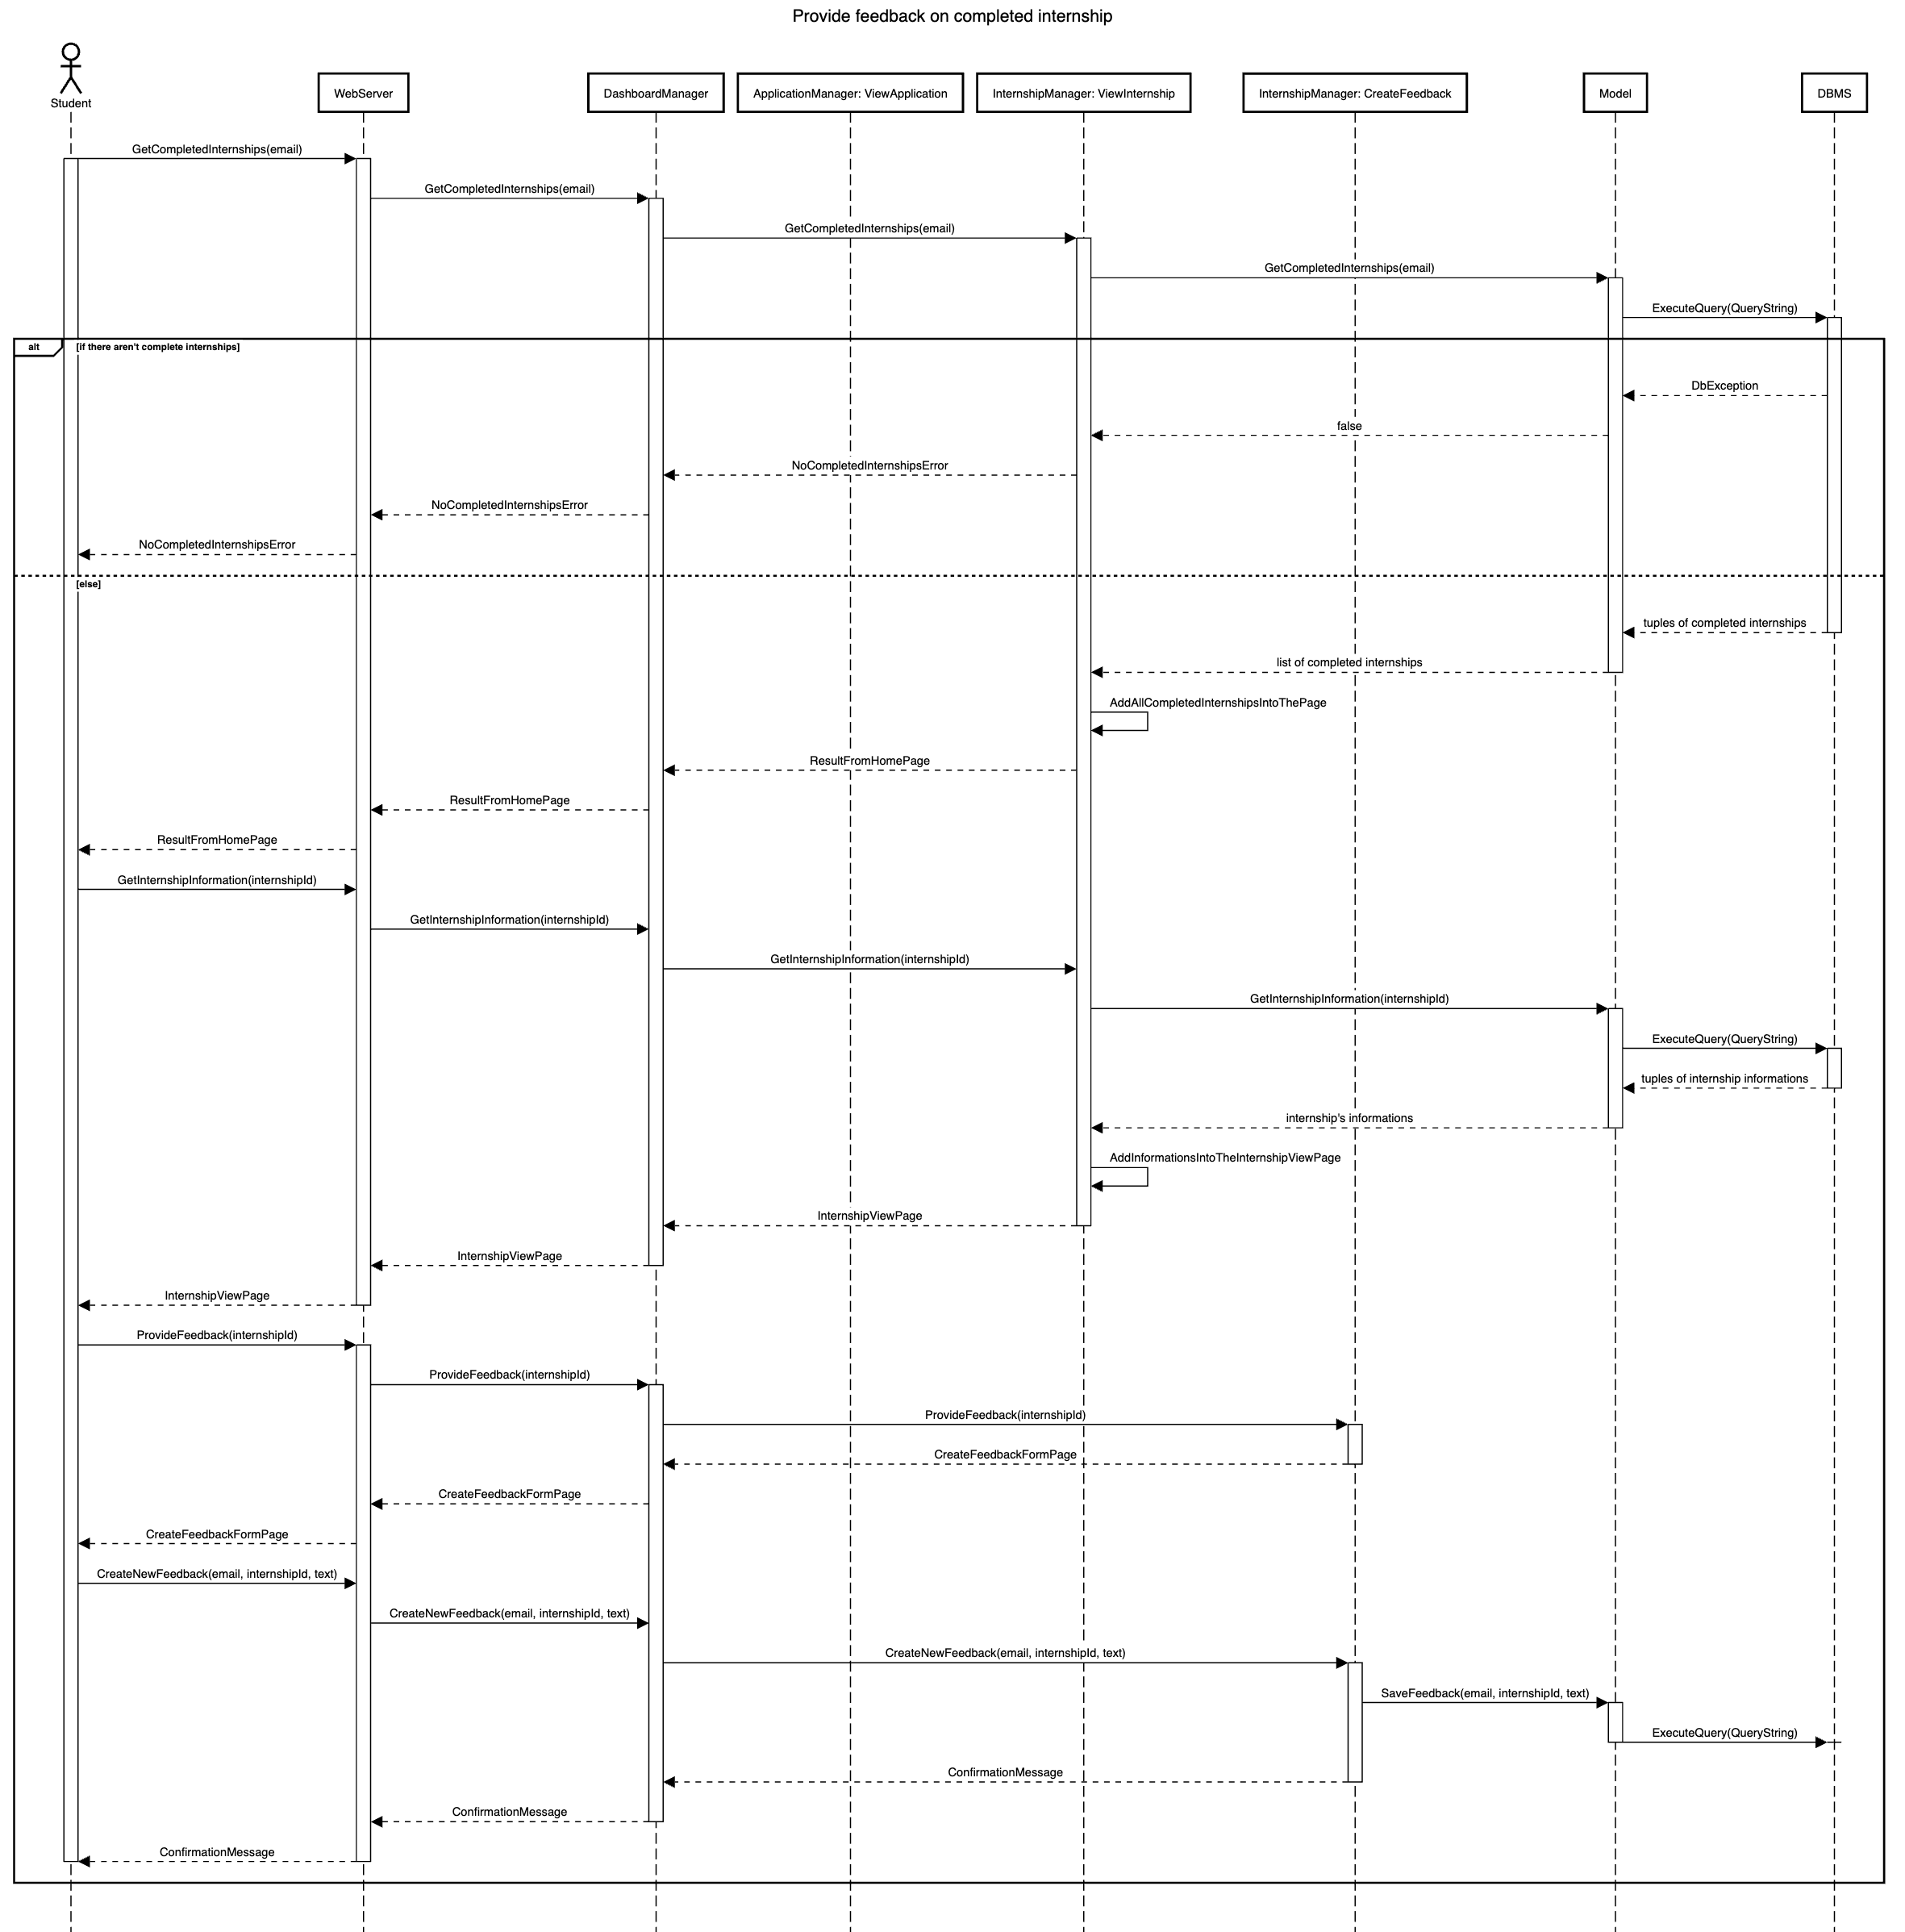
\includegraphics[width=0.8\linewidth]{DD/LaTeX/Images/RuntimeView/ProvideFeedback.png}
        \caption{Runtime view for 'Provide feedback on completed internships'.}
        \label{fig:runtime_ProvideFeedback}%
    \end{center}
\end{figure}

DESCRIPTION


\subsection{File complaints about internships}
\begin{figure}[H]
    \begin{center}
        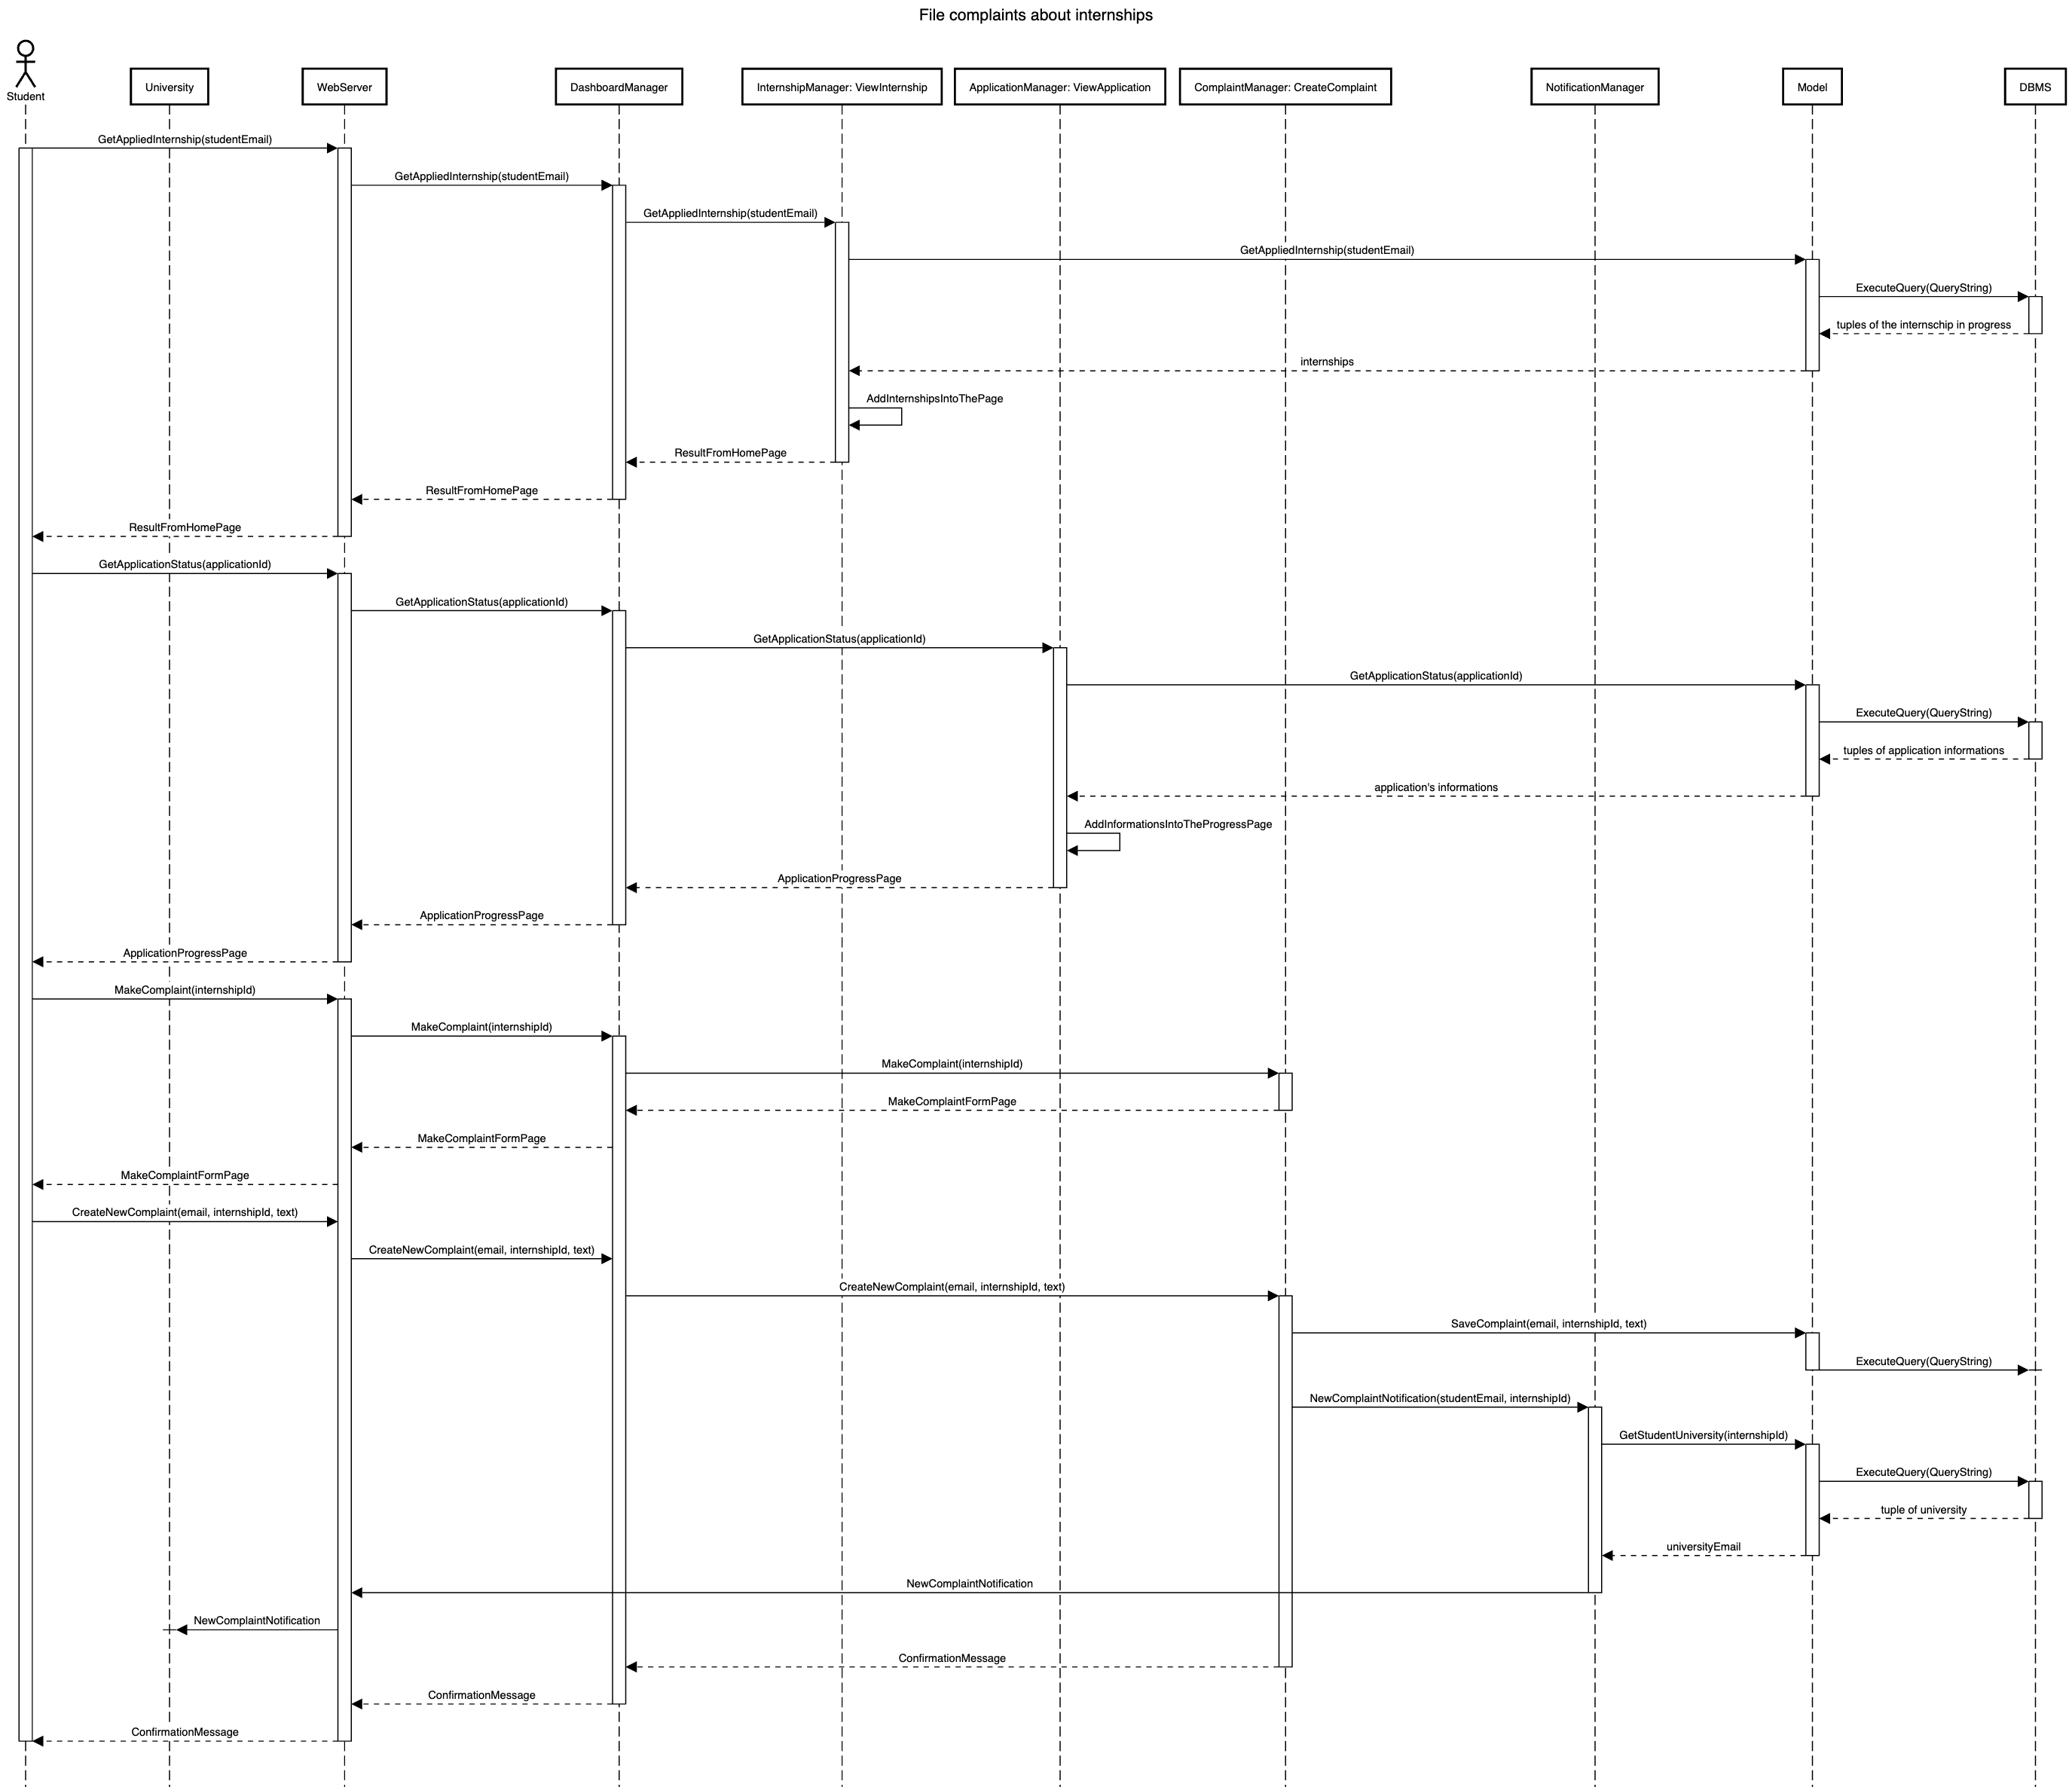
\includegraphics[width=0.8\linewidth]{DD/LaTeX/Images/RuntimeView/FileComplaints.png}
        \caption{Runtime view for 'File complaints about internships'.}
        \label{fig:runtime_FileComplaints}%
    \end{center}
\end{figure}

DESCRIPTION


\subsection{Create and publish internships}
\begin{figure}[H]
    \begin{center}
        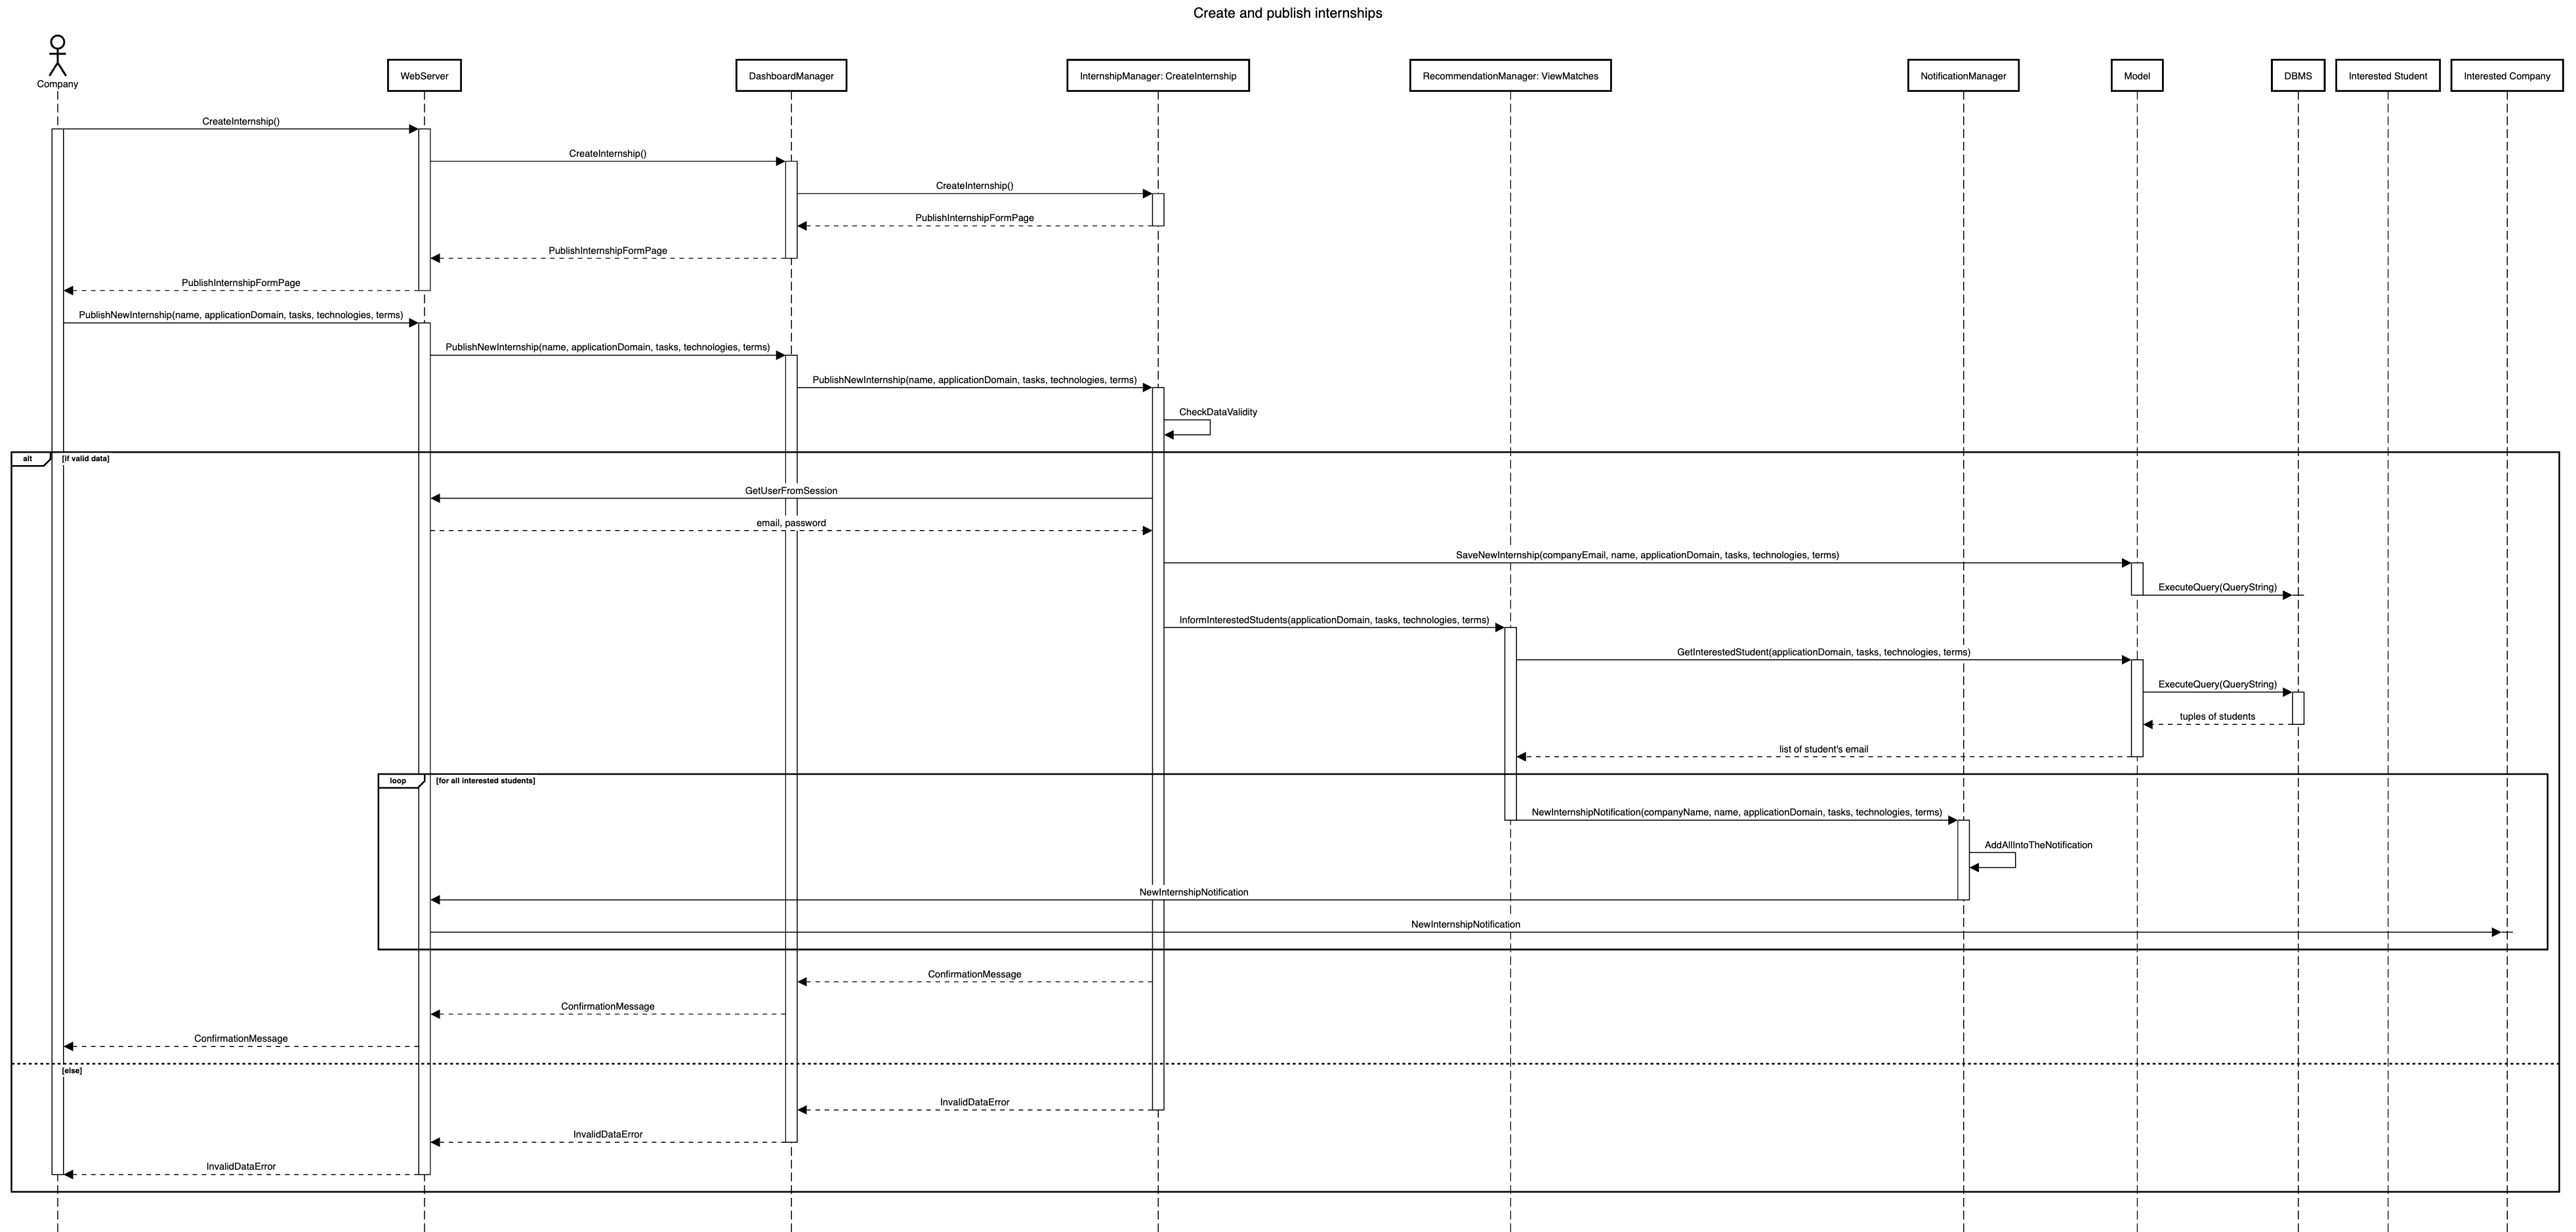
\includegraphics[width=0.8\linewidth]{DD/LaTeX/Images/RuntimeView/PublishInternship.png}
        \caption{Runtime view for 'Create and publish internships'.}
        \label{fig:runtime_PublishInternship}%
    \end{center}
\end{figure}

DESCRIPTION


\subsection{View and manage published internships}
\begin{figure}[H]
    \begin{center}
        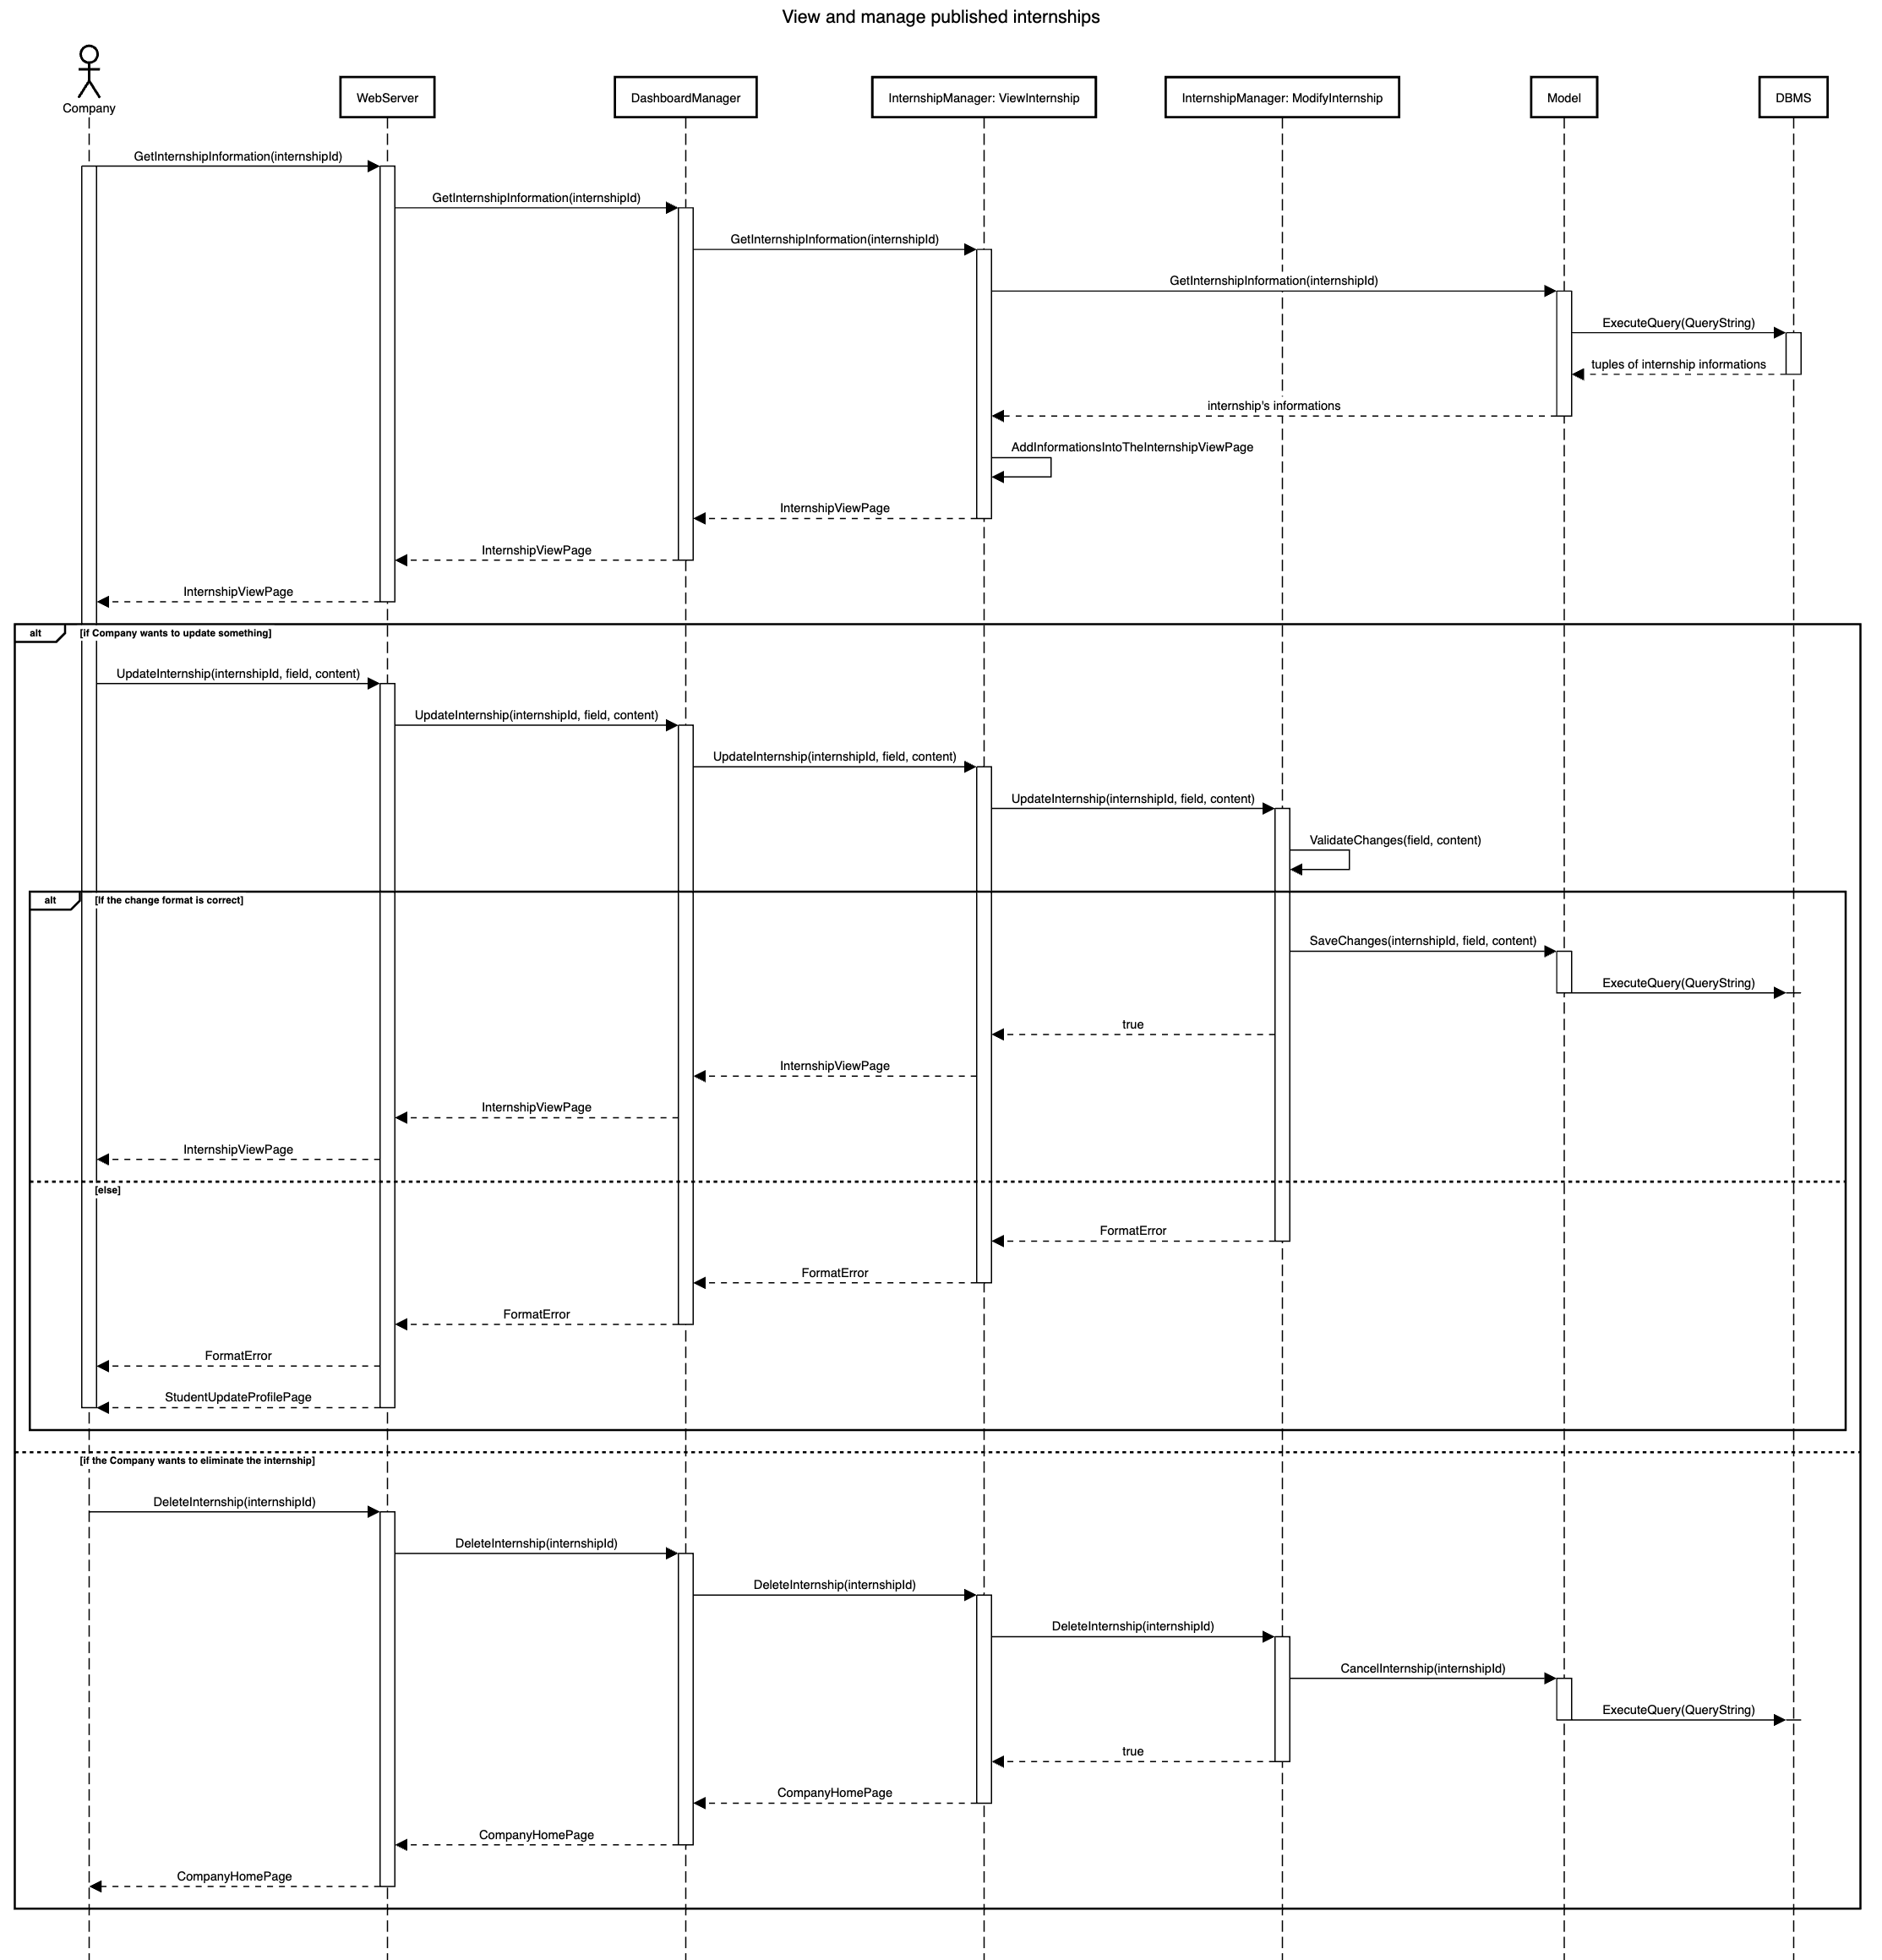
\includegraphics[width=0.8\linewidth]{DD/LaTeX/Images/RuntimeView/ManageInternships.png}
        \caption{Runtime view for 'View and manage published internships'.}
        \label{fig:runtime_ManageInternships}%
    \end{center}
\end{figure}

DESCRIPTION


\subsection{View recommended students for internships}
\begin{figure}[H]
    \begin{center}
        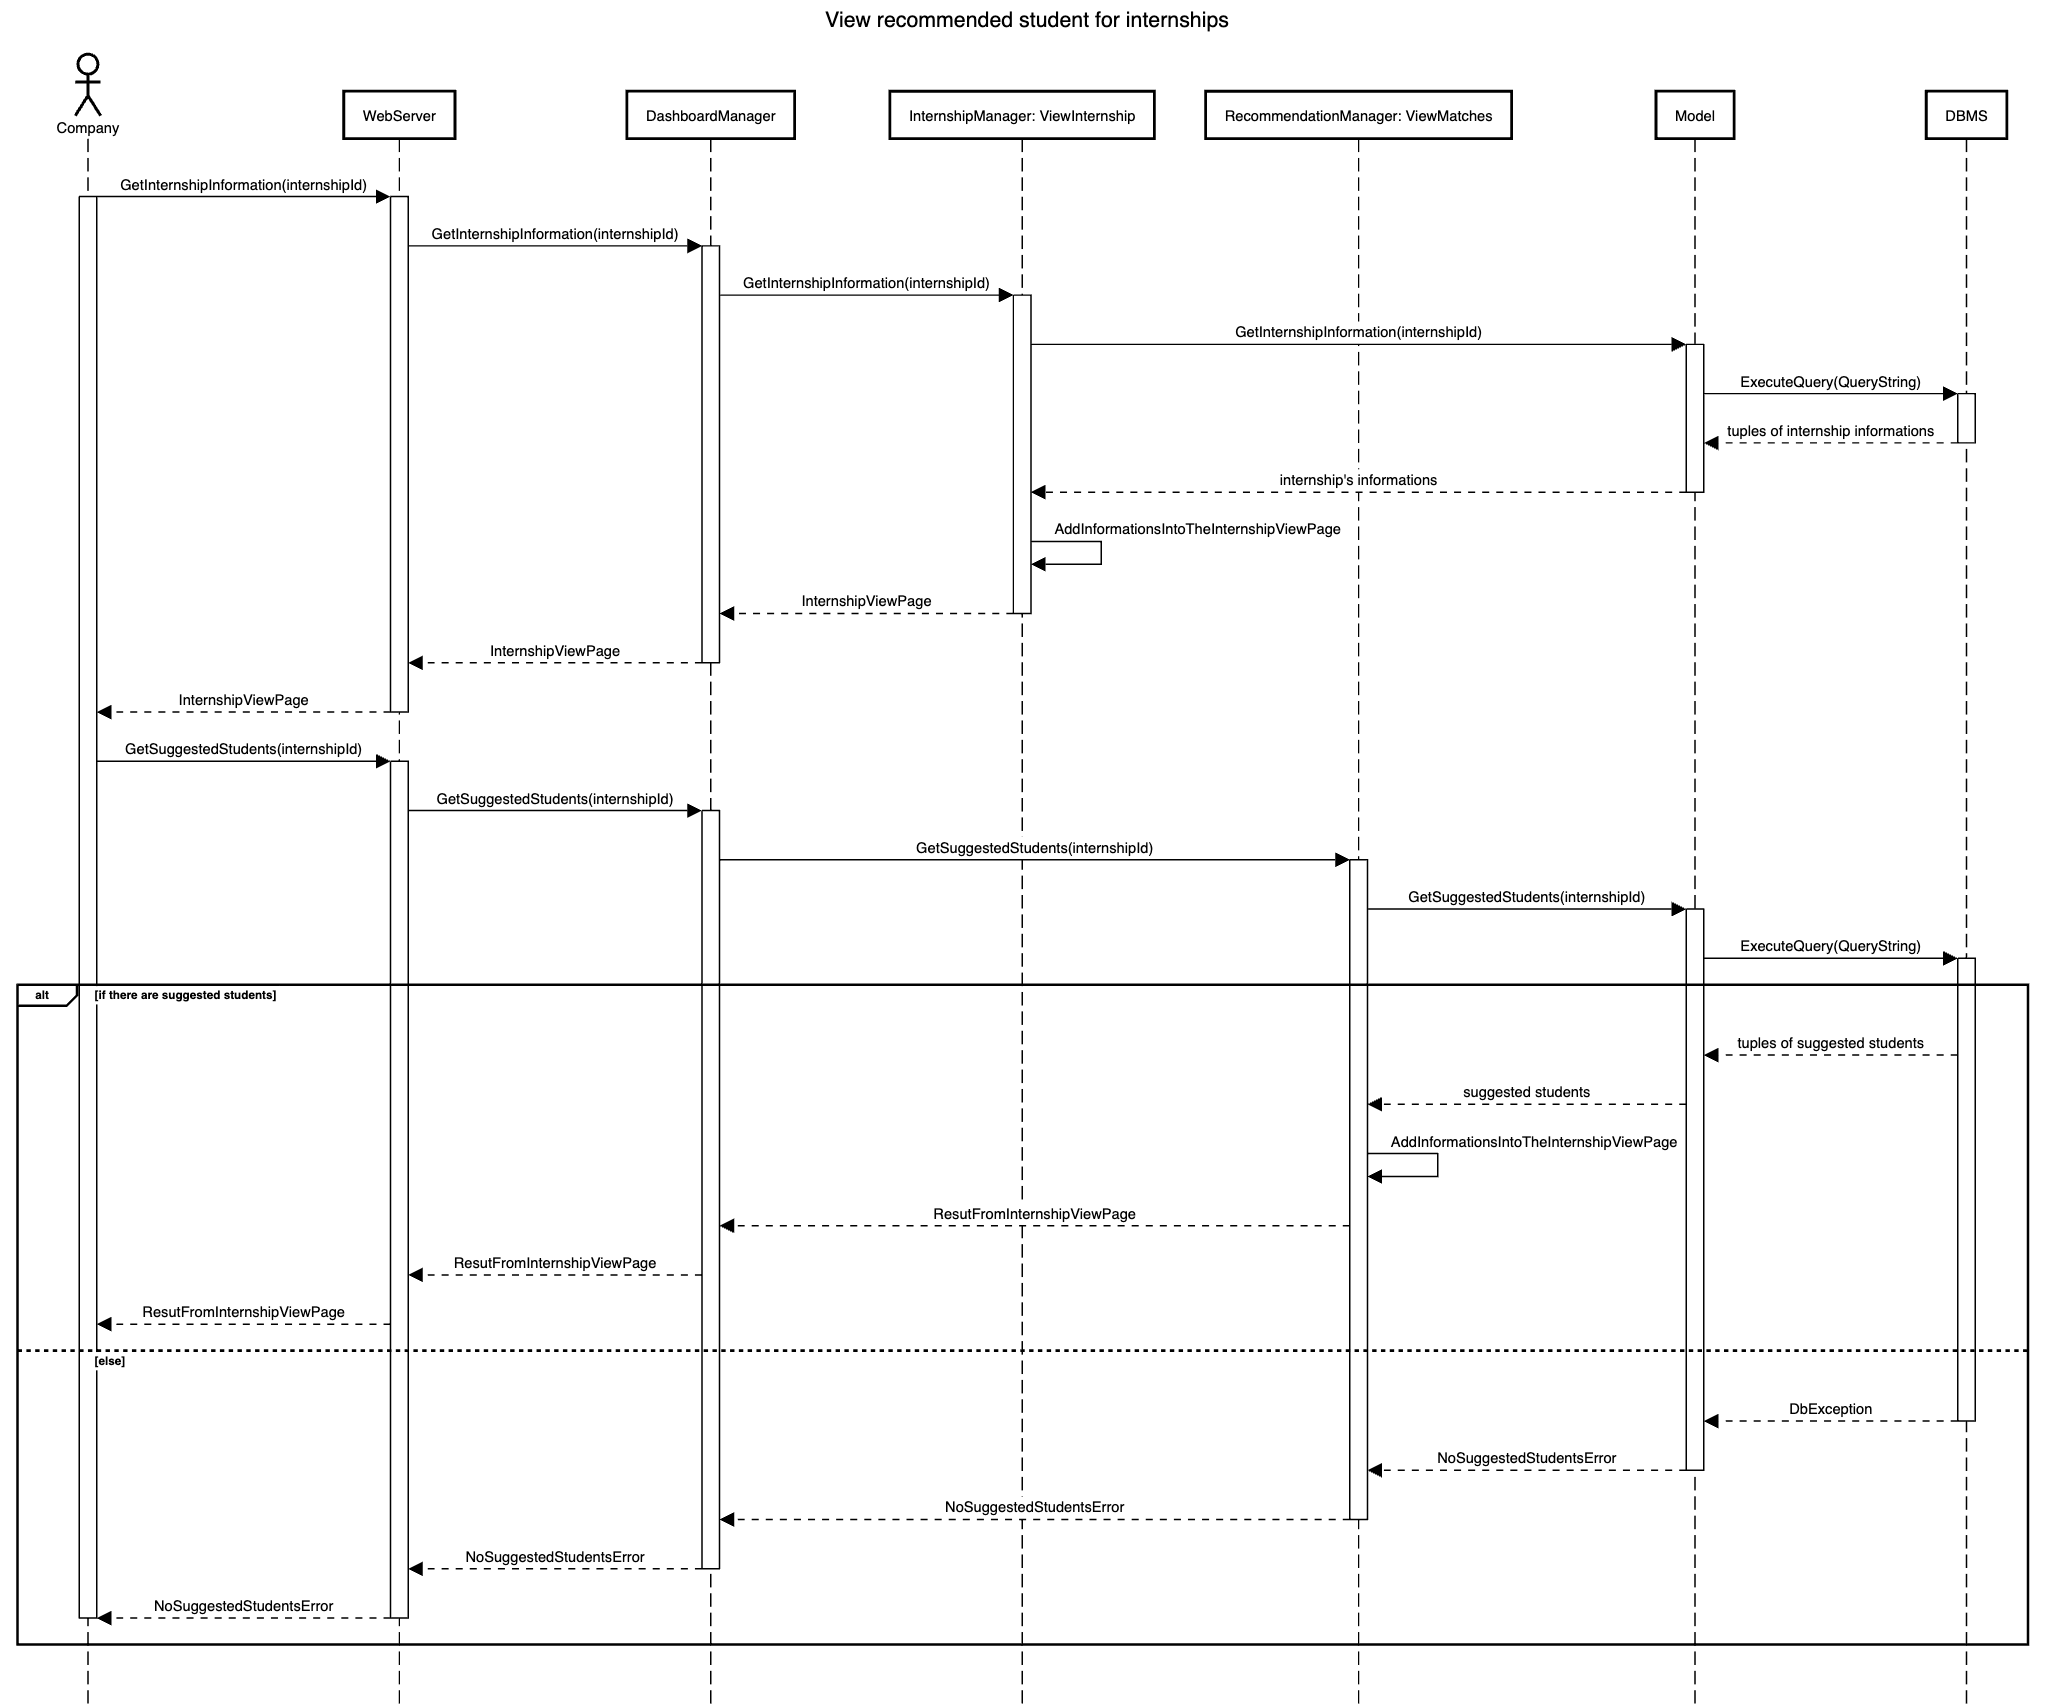
\includegraphics[width=0.8\linewidth]{DD/LaTeX/Images/RuntimeView/ViewRecommendedStudenst.png}
        \caption{Runtime view for 'View recommended students for internships'.}
        \label{fig:runtime_ViewRecommendedStudenst}%
    \end{center}
\end{figure}

DESCRIPTION


\subsection{Contact students for internships}
\begin{figure}[H]
    \begin{center}
        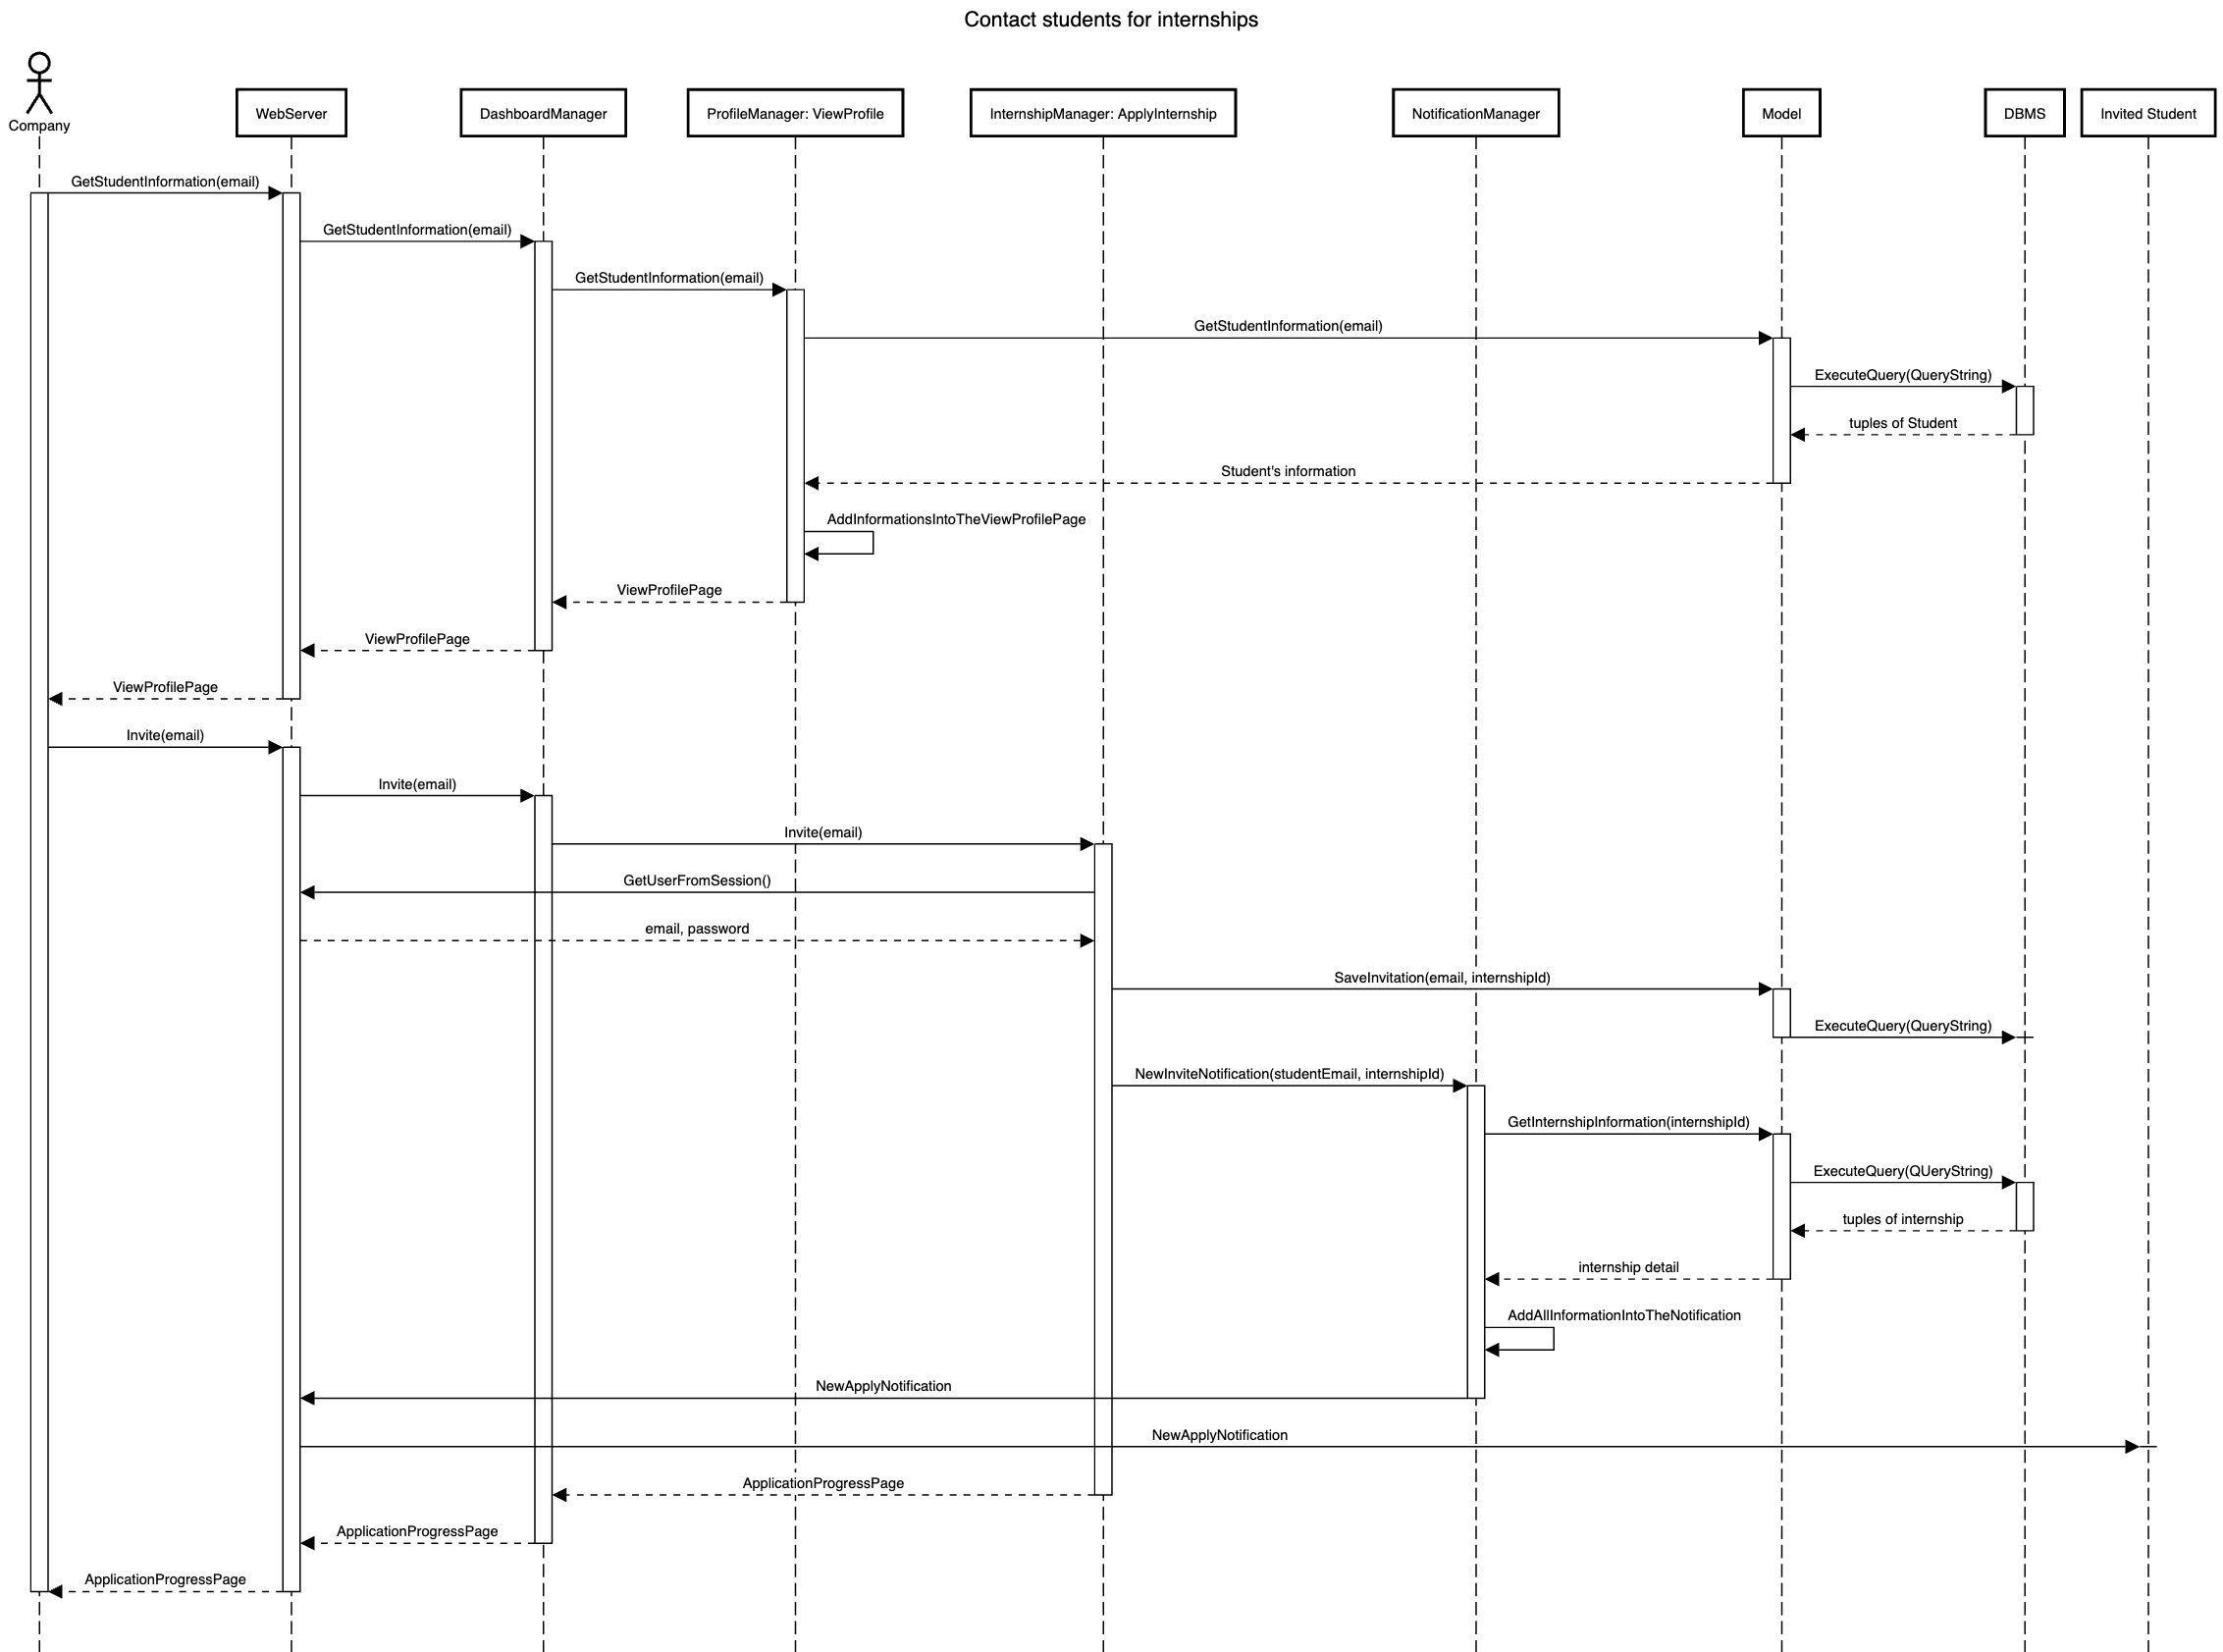
\includegraphics[width=0.8\linewidth]{DD/LaTeX/Images/RuntimeView/ContactStudent.png}
        \caption{Runtime view for 'Contact students for internships'.}
        \label{fig:runtime_ContactStudent}%
    \end{center}
\end{figure}

DESCRIPTION

\subsection{Accept student applications}
\begin{figure}[H]
    \begin{center}
        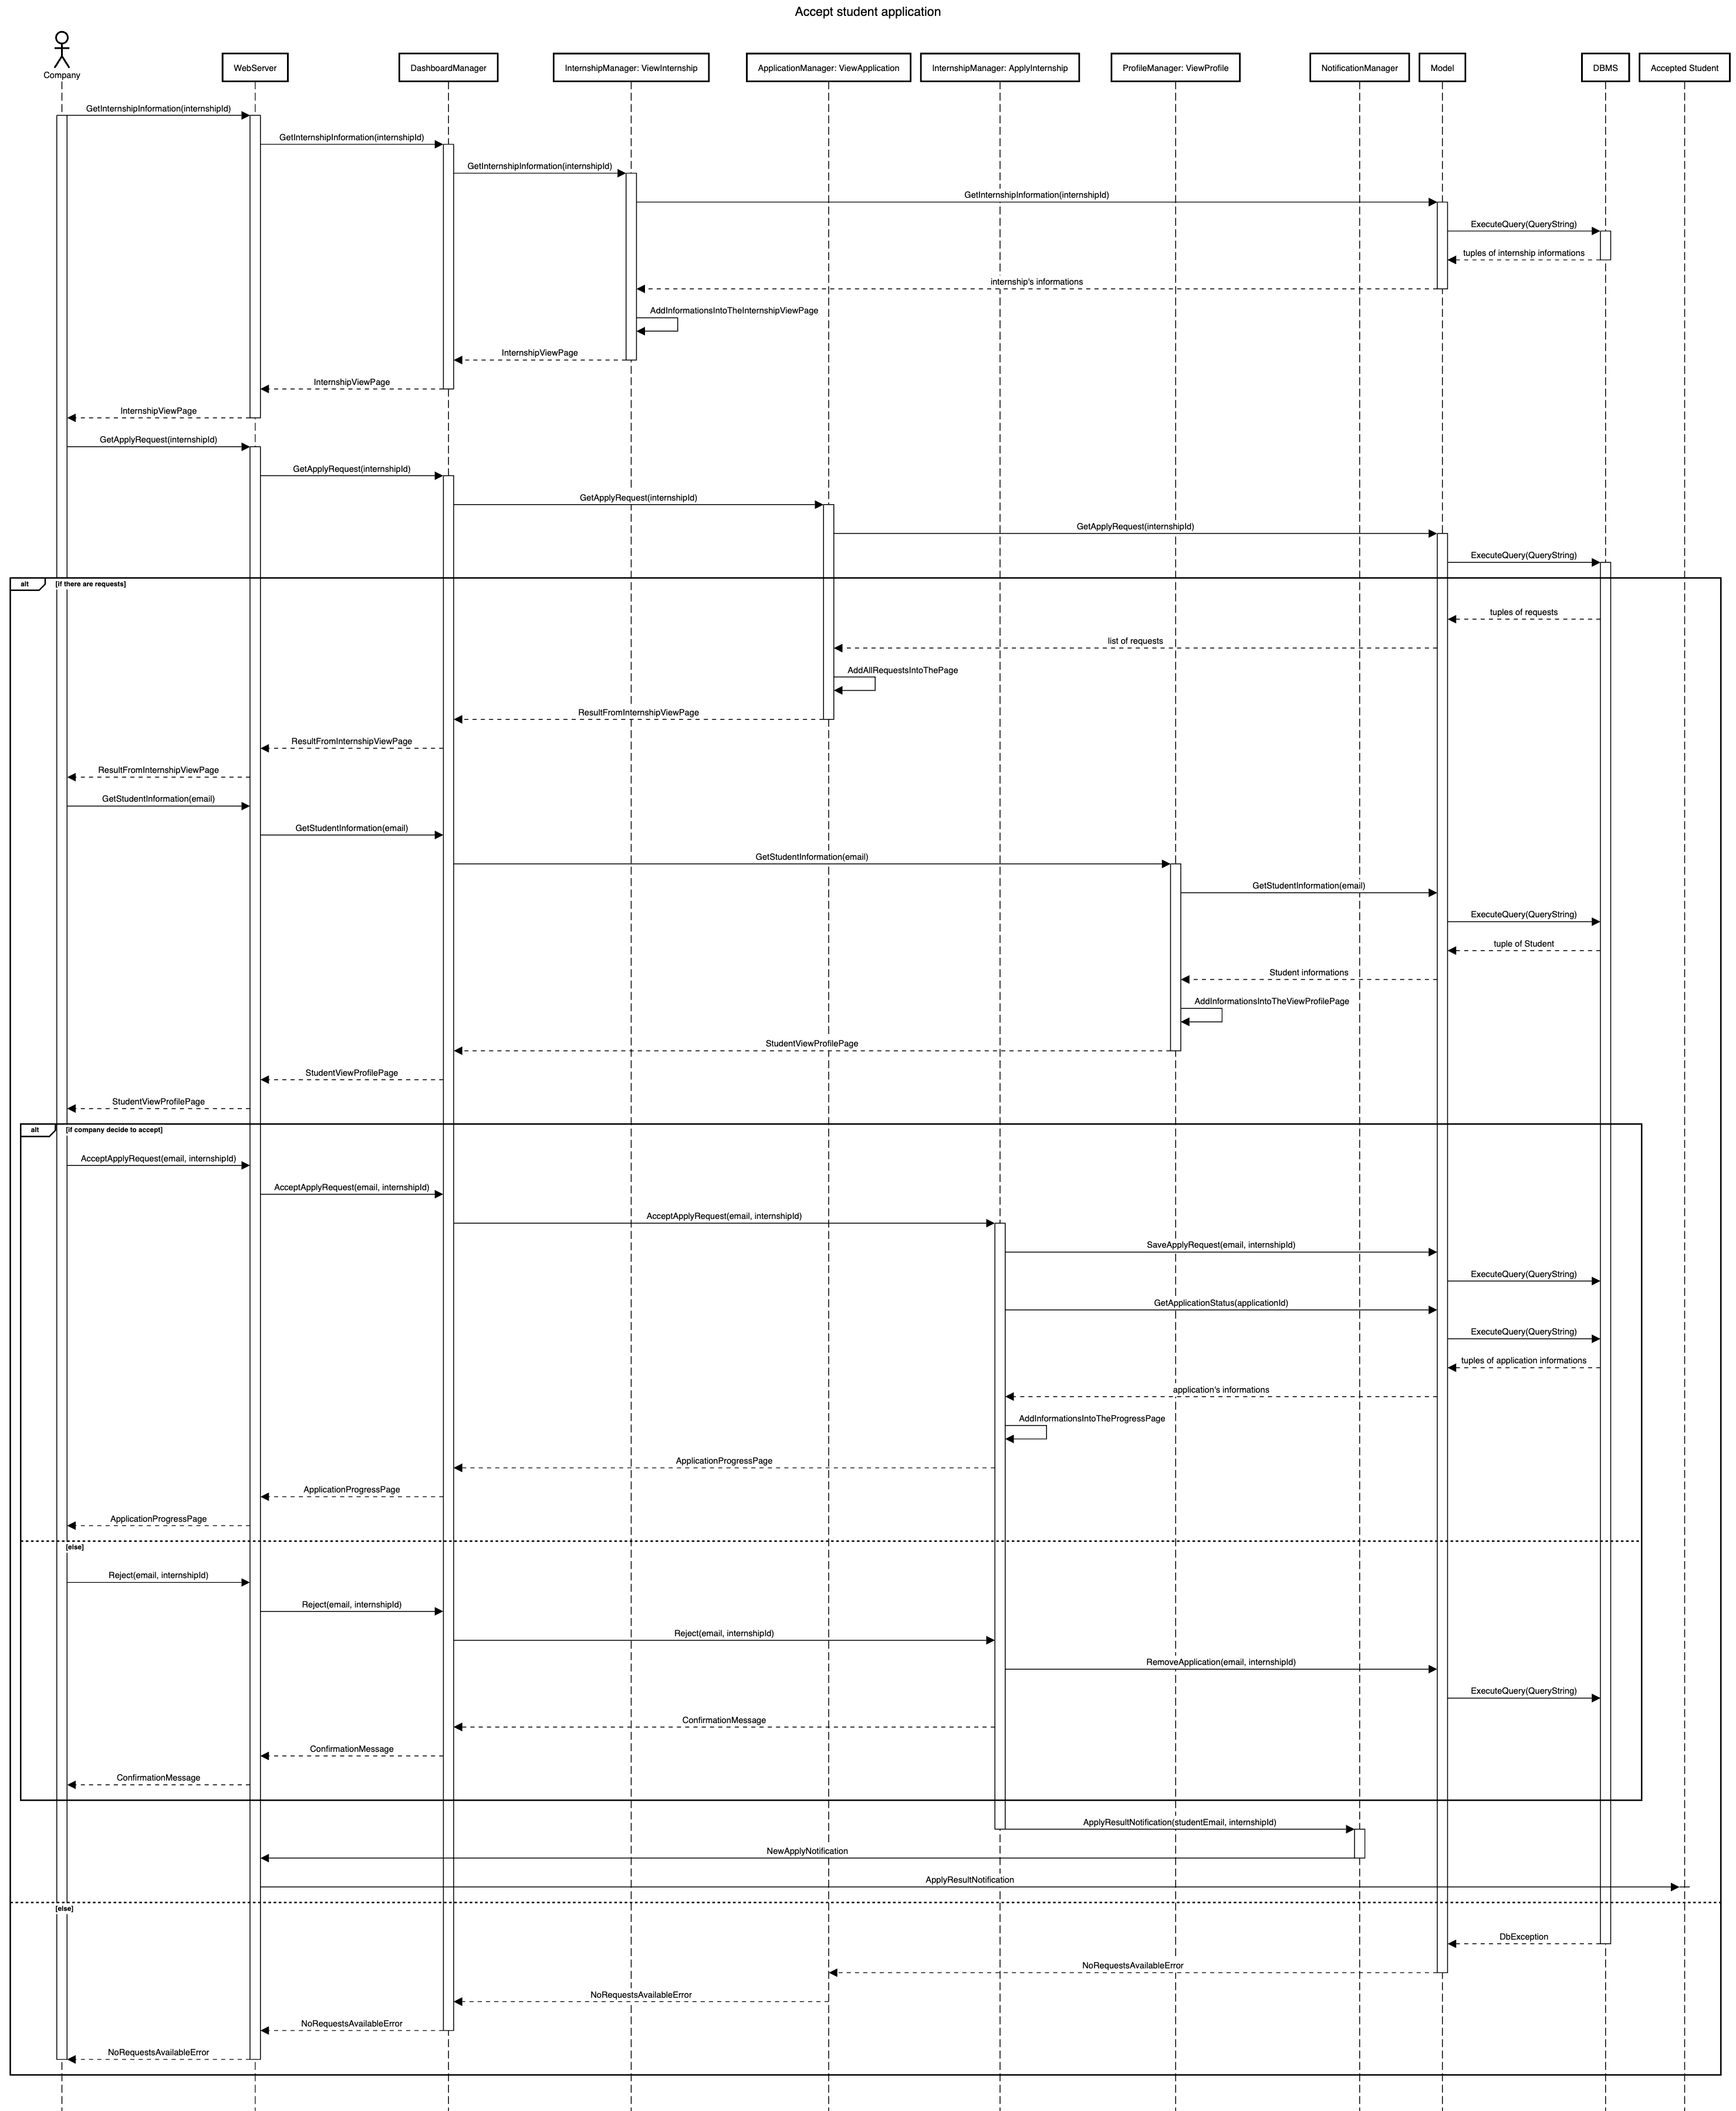
\includegraphics[width=0.8\linewidth]{DD/LaTeX/Images/RuntimeView/AcceptSTApplication.png}
        \caption{Runtime view for 'Accept student applications'.}
        \label{fig:runtime_AcceptSTApplication}%
    \end{center}
\end{figure}

DESCRIPTION


\subsection{Submit questionnaires for students}
\begin{figure}[H]
    \begin{center}
        \includegraphics[width=0.8\linewidth]{RuntimeView/}
        \caption{Runtime view for 'Submit questionnaires for students'.}
        \label{fig:runtime_modifybadge}%
    \end{center}
\end{figure}

DESCRIPTION


\subsection{Finalize the selection process}
\begin{figure}[H]
    \begin{center}
        \includegraphics[width=0.8\linewidth]{RuntimeView/}
        \caption{Runtime view for 'Finalize the selection process'.}
        \label{fig:runtime_modifybadge}%
    \end{center}
\end{figure}

DESCRIPTION


\subsection{Provide feedback on interns}
\begin{figure}[H]
    \begin{center}
        \includegraphics[width=0.8\linewidth]{RuntimeView/}
        \caption{Runtime view for 'Provide feedback on interns'.}
        \label{fig:runtime_modifybadge}%
    \end{center}
\end{figure}

DESCRIPTION


\subsection{File complaints about students}
\begin{figure}[H]
    \begin{center}
        \includegraphics[width=0.8\linewidth]{RuntimeView/}
        \caption{Runtime view for 'File complaints about students'.}
        \label{fig:runtime_modifybadge}%
    \end{center}
\end{figure}

DESCRIPTION


\subsection{Monitor the status of all internships}
\begin{figure}[H]
    \begin{center}
        \includegraphics[width=0.8\linewidth]{RuntimeView/}
        \caption{Runtime view for 'Monitor the status of all internships'.}
        \label{fig:runtime_modifybadge}%
    \end{center}
\end{figure}

DESCRIPTION


\subsection{Handle complaints from students or companies}
\begin{figure}[H]
    \begin{center}
        \includegraphics[width=0.8\linewidth]{RuntimeView/}
        \caption{Runtime view for 'Handle complaints from students or companies'.}
        \label{fig:runtime_modifybadge}%
    \end{center}
\end{figure}

DESCRIPTION


\subsection{Cancel problematic internships}
\begin{figure}[H]
    \begin{center}
        \includegraphics[width=0.8\linewidth]{RuntimeView/}
        \caption{Runtime view for 'Cancel problematic internships'.}
        \label{fig:runtime_modifybadge}%
    \end{center}
\end{figure}

DESCRIPTION


\subsection{Collect feedback from companies and students to improve matching}
\begin{figure}[H]
    \begin{center}
        \includegraphics[width=0.8\linewidth]{RuntimeView/}
        \caption{Runtime view for 'Collect feedback from companies and students to improve matching'.}
        \label{fig:runtime_modifybadge}%
    \end{center}
\end{figure}

DESCRIPTION


\subsection{Inform companies about available students matching their criteria}
\begin{figure}[H]
    \begin{center}
        \includegraphics[width=0.8\linewidth]{RuntimeView/}
        \caption{Runtime view for 'Inform companies about available students matching their criteria'.}
        \label{fig:runtime_modifybadge}%
    \end{center}
\end{figure}

DESCRIPTION


\subsection{Inform students about new internship opportunities}
\begin{figure}[H]
    \begin{center}
        \includegraphics[width=0.8\linewidth]{RuntimeView/}
        \caption{Runtime view for 'Inform students about new internship opportunities'.}
        \label{fig:runtime_modifybadge}%
    \end{center}
\end{figure}

DESCRIPTION





\section{Component Interfaces}
\label{sec:component_interfaces}%
\begin{itemize}
    \item \textbf{\textbf{Login}}
    \begin{itemize}

\item Login(\textit{String} nickname, \textit{String} password)
\end{itemize}
    \item \textbf{\textbf{SearchProfile}}


    \begin{itemize}

\item SearchUser(\textit{String} keyword)
\end{itemize}


    \item \textbf{\textbf{OpenProfile}}
    \begin{itemize}

\item SelectUser(\textit{String} nickname)

\end{itemize}


    \item \textbf{\textbf{RegistrationManager}}

\begin{itemize}
        \item CreateAnAccount()
        \item Registration(\textit{String} name, \textit{String} surname, \textit{String} nickname, \textit{String} mail, \textit{String} password, \textit{Boolean}  ED tick)
        \item Registration(\textit{String} name, \textit{String} surname, \textit{String} nickname, \textit{String} mail, \textit{String} password)
\end{itemize}

    \item \textbf{\textbf{Create Tournament}}

\begin{itemize}
        \item CreateATournament()
        \item TournamentInformation(\textit{String} tournament name, \textit{Date} subscription deadline, \textit{List\textless Educator\textgreater}  list of educators, \textit{Boolean} create badge tick)
        \item BadgeDetails(\textit{String} tournament name, \textit{String} badge name, \textit{String} description, \textit{String} rules of badge)
        \item SelectedBadge(\textit{String} tournament name, \textit{String} badge name)
        \item ChangeBadge(\textit{String} tournament name, \textit{String} badge name, \textit{String} description, \textit{String} rules of badge)
\end{itemize}

    \item \textbf{\textbf{Join Tournament}}
\begin{itemize}
        \item JoinTournament(\textit{String} tournament name)
\end{itemize}

    \item \textbf{\textbf{View Tournament}}

\begin{itemize}
        \item GetTournamentInformation(\textit{String} tournament name)
        \item SearchTournament(\textit{String} keyword)
\end{itemize}

    \item \textbf{\textbf{CreateBadge}}
\begin{itemize}

    \item BadgeDetails(\textit{String} tournament name, \textit{String} badge name, \textit{String} description, \textit{String} rules of badge)
\end{itemize}

    \item \textbf{\textbf{ModifyBadge}}

\begin{itemize}
        \item SelectedBadge(\textit{String} tournament name, \textit{String} badge name)
        \item ChangeBadge(\textit{String} tournament name, \textit{String} badge name, \textit{String} description, \textit{String} rules of badge)
\end{itemize}

    \item \textbf{\textbf{Model}}

\begin{itemize}
        \item CheckCredentials(\textit{String} nickname, \textit{String} password)
        \item GetEducatorTournaments(\textit{String} nickname)
        \item GetStudentTournaments(\textit{String} nickname)
        \item GetNewBattlesFromTournaments(\textit{List\textless Tournament\textgreater} list tournament, \textit{String} nickname)
        \item GetLastTournaments()
        \item GetRepositoryLink(\textit{String} tournament name, \textit{String} battle name, \textit{String} group name)
        \item GetAdditionalConfiguration(\textit{String} tournament name, \textit{String} battle name)
        \item SaveScore(\textit{Int}  score, \textit{String} tournament name, \textit{String} battle name, \textit{String} group name)
        \item CheckNickname(\textit{String} nickname)
        \item CheckMail(\textit{String} mail)
        \item SaveNewUserCredentials(\textit{String} name, \textit{String} surname, \textit{String} nickname, \textit{String} mail, \textit{String} password, \textit{Boolean}  ED tick)
        \item GetAllStudents()
        \item GetUser(\textit{String} nickname)
        \item GetUsers(\textit{String} keyword)
        \item GetDeadlineExpiration(\textit{String} tournament name)
        \item GetDeadlineExpiration(\textit{String} tournament name, \textit{String} battle name)
        \item GetRegistrationDeadline(\textit{String} tournament name, \textit{String} battle name)
        \item CheckBadgeNameDoesNotExists(\textit{String} tournament name, \textit{String} badge name)
        \item GetAllEducatorBadge(\textit{String} nickname)
        \item SaveNewBadge(\textit{String} tournament name, \textit{String} badge name, \textit{String} description, \textit{String} rules of badge)
        \item CheckBadgeBelongsToEducator(\textit{String} nickname, \textit{String} badge name)
        \item SaveChangedBadge(\textit{String} tournament name, \textit{String} badge name, \textit{String} description, \textit{String} rules of badge)
        \item GetTournamentName(\textit{String} tournament name)
        \item GetTournamentInformation(\textit{String} tournament name)
        \item GetTournamentFromSearch(\textit{String} keyWord)
        \item GetStudentTournaments(\textit{String} nickname)
        \item GetLastTournaments()
        \item SaveStudentAsTournamentPartecipant(\textit{String} tournament name, \textit{String} nickname)
        \item GetAllStudentsIntheTournament(\textit{String} tournament name)
        \item CheckStudentAlreadyJoinedTournament(\textit{String} tournament name, \textit{List\textless String\textgreater} list nicknames)
        \item CheckStudentAlreadyJoinedTouenament(\textit{String} tournament name, \textit{String} nickname)
        \item CheckGroupAlreadyJoined(\textit{String} tournament name, \textit{String} battle name, \textit{String} group name)
        \item CheckGroupNumber(\textit{String} tournament name, \textit{String} battle name, \textit{String} group name)
        \item SaveGroupIntheBattleList(\textit{String} tournament name, \textit{String} battle name, \textit{String} group name)
        \item CheckBattleName(\textit{String} tournament name, \textit{String} battle name)
        \item GetBattleInformation(\textit{String} tournament name, \textit{String} battle name)
        \item CheckGroupName(\textit{String} tournament name, \textit{String} battle name, \textit{String} group name)
        \item CheckGroupParticipants(\textit{String} tournament name, \textit{String} battle name, \textit{String} group name)
        \item AddStudentToGroup(\textit{String} nickname, \textit{String} tournament name, \textit{String} battle name, \textit{String} group name)
        \item CreateNewBattle(\textit{String} tournament name, \textit{String} battle name, \textit{String} code kata, \textit{Int}  minimum member per group, \textit{Int}  maximum member per group, \textit{Date} registration deadline, \textit{Date} final submission deadline, \textit{List\textless String\textgreater} list additional configuration for scoring, \textit{String} repository link)
        \item CheckStudentAlreadyJoinedBattle(\textit{String} battle name, \textit{String} tournament name, \textit{String} nickname)
        \item GetEducatorsName(\textit{List\textless Educators\textgreater} list of educators)
        \item SaveNewTournament(\textit{String} tournament name, \textit{String} subscription deadline, \textit{List\textless Educators\textgreater} list of educators)
\end{itemize}

    \item \textbf{\textbf{CreateBattle}}

\begin{itemize}
        \item NewBattle(\textit{String} tournament name)
        \item CreateBattle(\textit{String} battle name, \textit{String} code kata, \textit{Int}  minimum member per group, \textit{Int}  maximum member per group, \textit{Date} registration deadline, \textit{Date} final submission deadline, \textit{List\textless String\textgreater} list additional configuration for scoring)
\end{itemize}

\end{itemize}

\begin{itemize}
    \item \textbf{\textbf{JoinBattle}}
\begin{itemize}
    \item ChooseBattle(\textit{String} tournament name, \textit{String} battle name)
    \end{itemize}


    \item \textbf{\textbf{CreateGroup}}

\begin{itemize}
        \item CreateGroupAndInvitation(\textit{String} tournament name, \textit{String} battle name, \textit{String} group name, \textit{List\textless String\textgreater} list nicknames)
        \item acceptInvitation(Student student, \textit{String} tournament name, \textit{String} battle name, \textit{String} group name)
        \item rejectInvitation(Student student, \textit{String} tournament name, \textit{String} battle name, \textit{String} group name)
        \item JoinBattle(\textit{String} tournament name, \textit{String} battle name, \textit{String} group name)
\end{itemize}

    \item \textbf{\textbf{ViewBattle}}
    \begin{itemize}
        \item GetBattleInformation(\textit{String} tournament name, \textit{String} battle name)
\end{itemize}

    \item \textbf{\textbf{EndBattle}}
\begin{itemize}
        \item StartFinalBattleTimer(\textit{String} tournament name, \textit{String} battle name, \textit{Date} final submission deadline)
\end{itemize}

    \item \textbf{\textbf{NotificationManager}}

\begin{itemize}
        \item ChosenEducatorNotification(\textit{String} nickname, \textit{String} tournament name)
        \item NewBattleNotification(\textit{String} nickname, \textit{String} tournament name, \textit{String} battle name)
        \item NewTournamentNotification(\textit{String} nickname, \textit{String} tournament name)
        \item SendInvitation(\textit{String} nickname, \textit{String} tournament name, \textit{String} battle name, \textit{String} group name)
\end{itemize}

    \item \textbf{\textbf{EvaluationManager}}

\begin{itemize}
        \item AnalyzeSourceCode(\textit{String} tournament name, \textit{String} battle name, \textit{String} group name)
        \item ScoreAssignment(\textit{Int}  score, \textit{String} tournament name, \textit{String} battle name, \textit{String} group name)
\end{itemize}

    \item \textbf{\textbf{DashboardManager}} (contains all the interfaces belonging to other managers, apart from NotificationManager and Model)

    \item \textbf{\textbf{WebServer}} (contains all the interfaces belonging to other managers, apart from NotificationManager and Model)
    \begin{itemize}
        \item GetSessionFromUser()
        \item AddUserToTheSession(\textit{String} nickname, \textit{String} password)
\end{itemize}

\end{itemize}


\section{Selected Architectural Styles and Patterns}
\label{sec:selected_Srchitectural_styles_patterns}%

CodeKataBattle will be developed over a \textbf{3-Tier architecture}, which is a software application architecture that organizes applications into three logical and physical computing tiers. Each tier runs on its own infrastructure, so the complexity of the system is reduced, its flexibility and scalability is enhanced. Each tier may be developed simultaneously by separate teams of developers and can be updated or scaled as needed without impacting the other tiers.
\\
The system is modularized over three independent tiers:
\begin{itemize}
    \item \textbf{Presentation Tier:} this is the top-level tier, that directly interacts with the Users. Its goal will be to collect the Users’ inputs and show them the outputs produced by the lower tiers. 
    \item \textbf{Application Tier:} this is the middle level tier. The Application Tier processes the Users’ requests that arrive from the Presentation Tier, perform the necessary computation, even retrieving or storing data on the Data Tier, and computes that data in order to complete specific tasks requested by the Users. This tier needs to handle several requests by different Users simultaneously, while guaranteeing the security and integrity of the stored data.
    \item \textbf{Data Tier:} this is the lowest level tier. The Data Tier stores, retrieves and manages data used or produced by the Application Tier by the DataBase System’s APIs.
\end{itemize}

For a more detailed description of the tiers and their components, please refer to \ckbautoref{sec:deployment_view}.\\
The behavior of the system will be mostly as a \textbf{Client-Server architecture}, in which the Client represents the front-end user interface, as it is the connection point between the final Users of the system and the system itself, meanwhile the Server represents the backend platform, as it elaborates the Users’ requests, computes and shows the answers. In a pure Client-Server architecture, the Server is always the one to make the request, while the server is a passive element, which handles and elaborates the requests of the Client and returns the answers to them. In some cases, such as when the process of sending the notifications or the interaction with the External Tools, the Server needs to perform operations without being invoked by the Client first, which makes it an active component and having a more Event Driven behavior.
\\
The Client-Server interactions are performed through \textbf{REST APIs}, a set of commands commonly used in the context of web transactions. The \textit{Representational State Transfer} consists in the use of a stateless Server, that means that the Client is the component that needs to communicate the state of the transaction to the Server. This approach allows the Server to be more scalable and helps with handling many requests that concern different states simultaneously. The components communicate by transferring a representation of a resource in a format that the Server is able to process, this allows the usage of HTTP protocol to share data and to encode those using the JSON format.
\\
The implementation of CKB will follow the \textbf{Model-View-Controller} pattern, which is a software design pattern that splits the software into three elements interconnected with each other: 
\begin{itemize}
    \item \textbf{Model:} contains the methods that manage the data. It provides methods for saving, retrieving and manipulating data from the database.
    \item \textbf{View:} the view is the part that concerns the visual representation of the data for the final user.
    \item \textbf{Controller:} acts as a connection point between the view and the model. The controller handles the users’ interactions with the view and processes the operations.
\end{itemize}

\section{Other Design Decisions}
\label{sec:other_design_decisions}%

\subsection{Availability}
The introduction of load balancing and replication mechanisms significantly enhances the reliability and availability of our system. Load balancing optimizes resource utilization by distributing requests evenly across servers, preventing performance bottlenecks.\\ Concurrently, replication ensures fault tolerance by duplicating essential data and services. This redundancy minimizes the impact of potential failures, fortifying our system to maintain consistent data management and service availability even in challenging scenarios.

\subsection{Scalability}
Microservices architecture, at its core, is meticulously crafted to be both independently deployable and inherently scalable. This design philosophy enables each microservice to be deployed autonomously, facilitating swift updates and modifications without disrupting the entire system. Beyond this, the scalability aspect of microservices empowers our system to gracefully handle increased demands by efficiently scaling specific services.


\subsection{Notification Handling}
Notification management plays a pivotal role in the CKB system, influencing every stage from Tournament, Battle or STG creation to their conclusion. Notifications in CKB are orchestrated to reach users upon login or, if a User is already logged in, immediately when they become available. This approach guarantees that Users are promptly informed about key events, such as Tournament, Battle or STG creation. 

\subsection{Ease of Deployment} 
The adoption of microservices architecture introduces a notable advantage in ease of deployment. This methodology empowers the implementation of changes to individual services independently, allowing for seamless deployment without impacting the entire system. In the event of issues, the microservices approach facilitates swift identification, isolation, and correction, eliminating the need to halt the entire system. This deployment flexibility not only accelerates the release of updates but also enhances the system's resilience and agility, enabling efficient troubleshooting and maintenance processes.

\subsection{Data Storage} 
To enhance operational efficiency and simplify data management, we've chosen a unified DBMS containing information about Users, Tournaments, Group, Badges and Battles. This approach reduces the time and complexity associated with retrieving and updating data, leveraging interconnected relationships among these components.